%Root main.tex
%---------------------------------------------------------------------------
%第2章　aaa
%---------------------------------------------------------------------------

\chapter{シミュレーション}
\label{chap:シミュレーション}

\section{シミュレーション}
本シミュレーションでは，連系リアクトルなし3相系統連系システムにおいて，定常運転時，系統擾乱発生時及び，アンノミナル時の出力応答の確認を行う．制御手法として，外乱補償型シングルレートデッドビート制御，外乱補償型マルチサンプリングデッドビート制御を適用する．本シミュレーションでは，系統電圧実行時が系統擾乱によって80\%瞬時低下する場合を想定し，インダクタ電流$I_{L1}$の応答を確認する．回路シミュレータはPSIMを用いた．本シミュレーションのパラメータを表\ref{Tab3.1}に示す．

\begin{table}[ht]
    \centering
    \caption{系統連系システムのパラメータ}
    \begin{tabular}{c|c|c}\hline\hline
         Condition          &Parameter  &Value\\ \hline
         Sampling frequency & $f_{s}$[kHz]   & 100 \\
         Carrier frequency  & $f_{c}$[kHz]   & 100 \\
         Nominal capacity   & $P$[MVA]       & 1.0 \\
%         Grid Voltage       & $V_{s}$[V_{rms}]   & 400 \\
         Operating frequency& $f$[Hz]       & 50 \\
         Dc power supply    & $E_{dc}$[V]  & 1200 \\
%         Filter inductor    & $L_{1}$[$\si{\mu }$H]   & 51 \\
%         Filter capacitor   & $C$[$\si{\mu }$F]       & 995 \\
%         Interconnection inductor & $L2$[$\si{\mu }$H] & 51 \\ \hline
    \end{tabular}
    \label{Tab3.1}
\end{table}

評価指標として，定常運転時の出力電流 Il1 の全高調波歪成分 [\%](THD:Total Har-monic Distriction) に関して評価を行った.  全高調波歪成分は，値が低ければ高調波成分の含有率が低く波形の精度が高いと評価できる．\par

 THDを求めるための式を以下に示す．なお，$I_{L1}$は基本波の実効値，$I_{L1n}$はn次高調波の実行値を表す．
\begin{align}
    THD=\frac{\sqrt{\sum_{n-2}^{\infty}-I^2_{L1n}}}{I_{L1}} \label{eq8}
\end{align}

FRT要件よりTHDは5.0\%以下が運転条件となっている．
表\ref{Tab3.2}にアンノミナル条件時のパラメータを示す．
\begin{table}[htb]
\centering
  \caption{パラーメータの変更パターン}
  \begin{tabular}{c|c|c|c}  \hline\hline 
    \multirow{2}{*}{Condition}& \multicolumn{3}{|c}{Parameter} \\  \cline{2-4}
     & $L_{1}$ & $C$  & $L_{2}$\\  \hline 
%    ノミナル時 & $51 \si{\mu }$H & $995 \si{\mu }$F & $51 \si{\mu }$H \\ 
    パターン1 & 1.5 mH & 2.0 mF & 0.2 mH \\ 
    パターン2 & 0.35 mH & 200 $\mu $F & 0.002 mH\\ \hline
  \end{tabular}
  \label{Tab3.2}
\end{table}

\section{シミュレーション結果}
\subsection{ノミナル検証}
外乱補償型シングルレートデッドビート制御の際の定常運転時と系統擾乱発生時の出力応答を示す．

\begin{figure}[ht]
    \center
    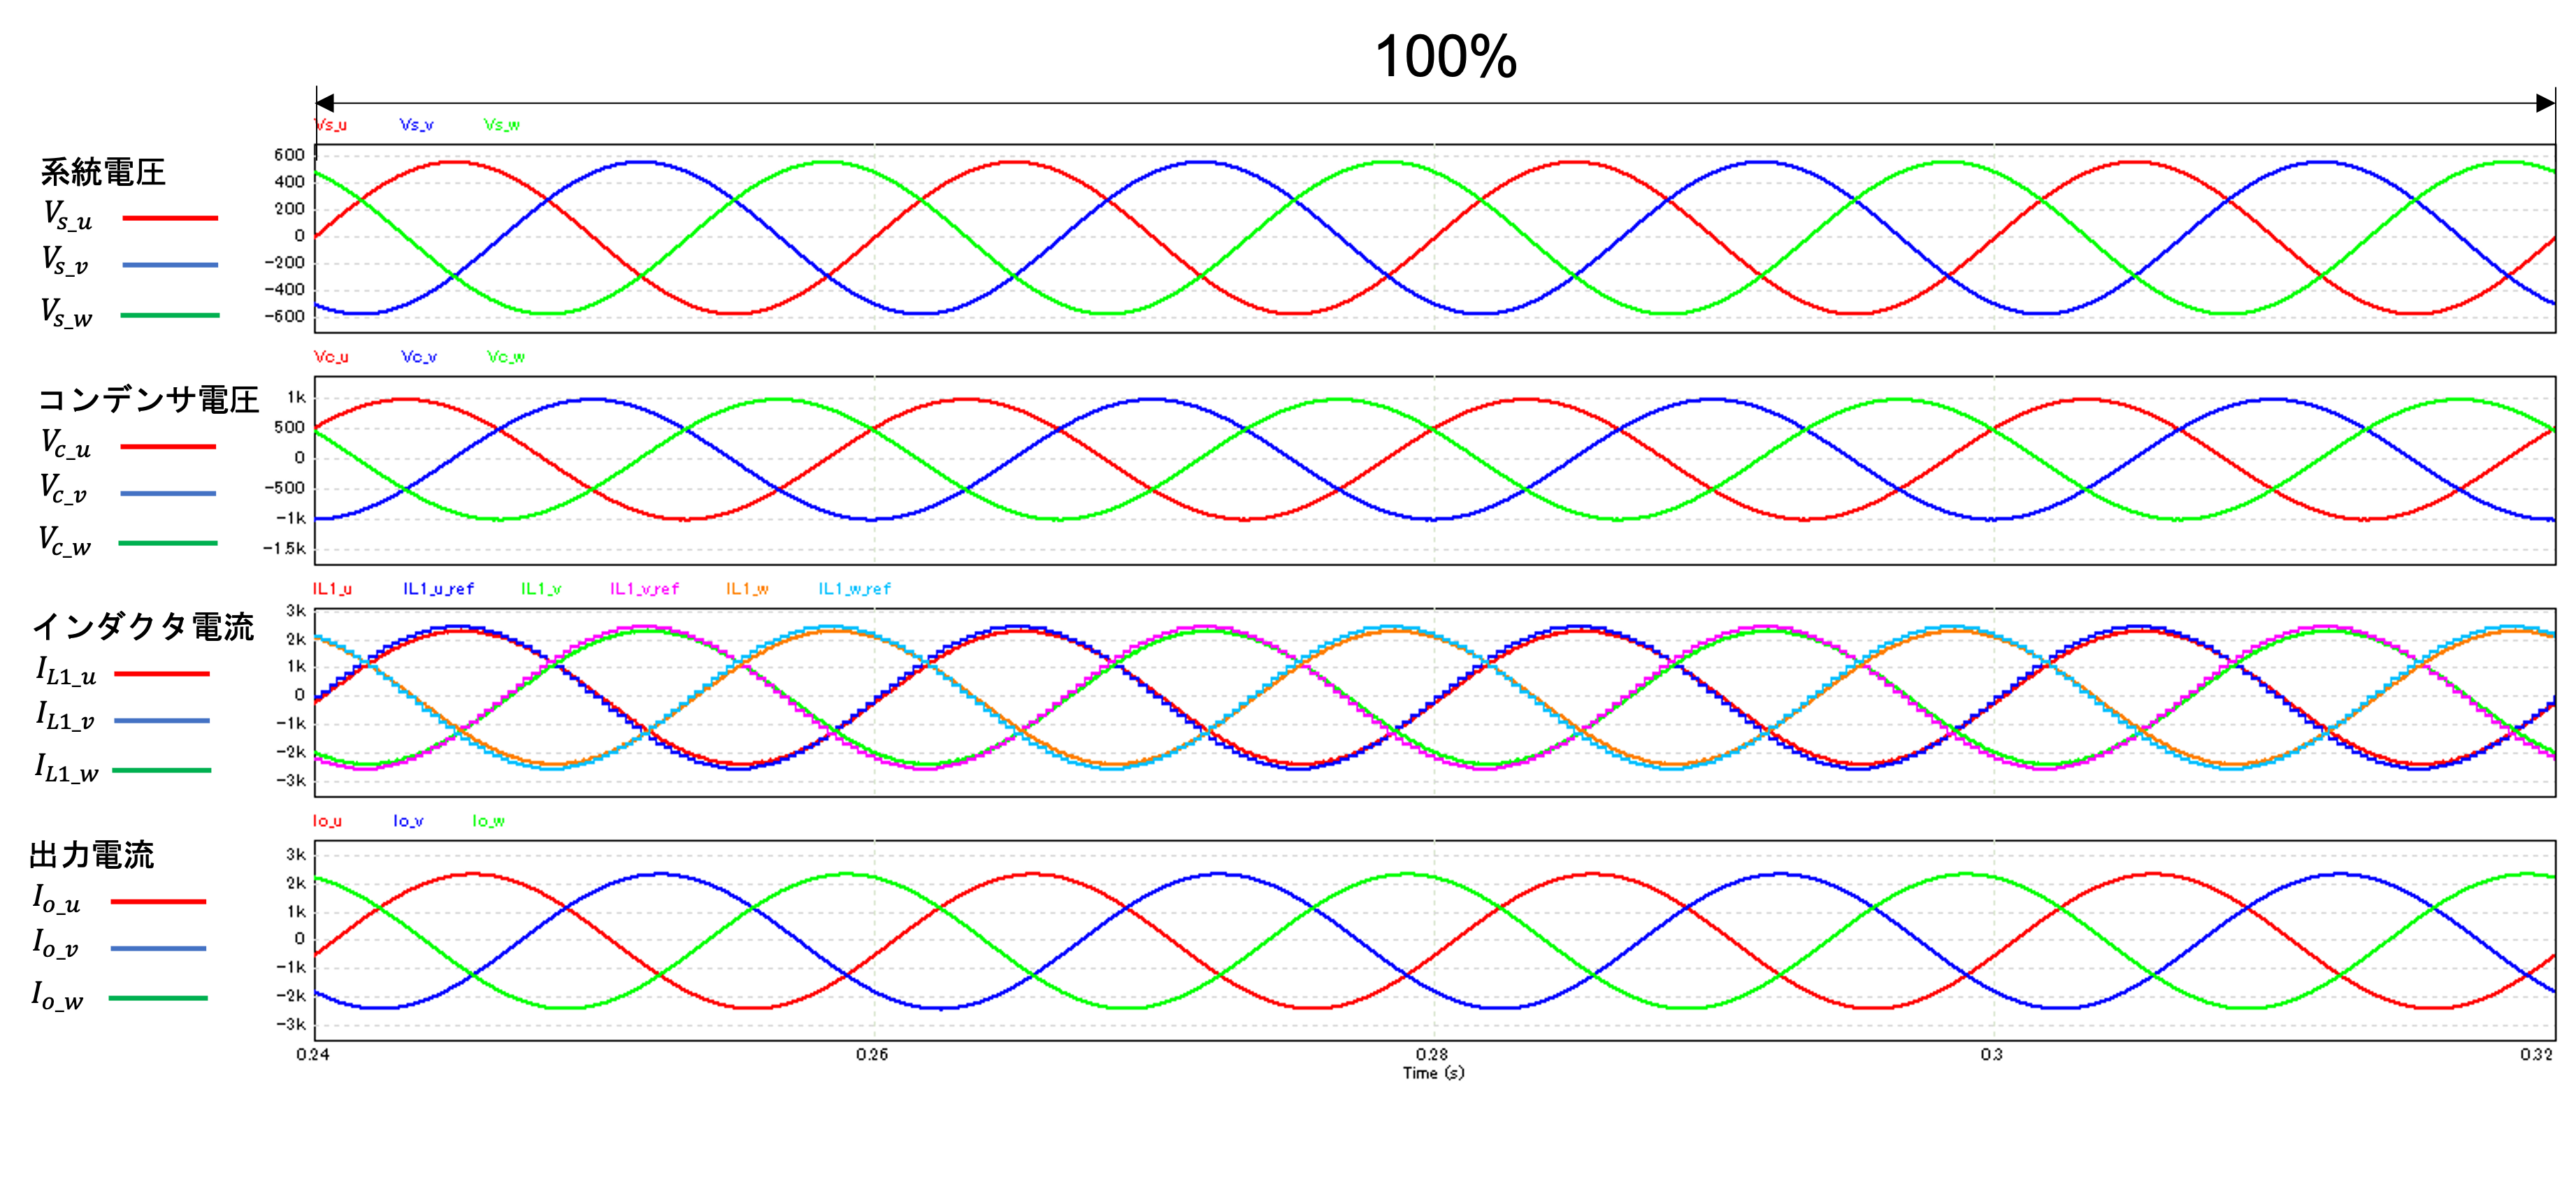
\includegraphics[width=140mm]{image/chapter3/Fig3.1.png}
    \caption{定常運転時の出力波形}
    \label{Fig3.1}
\end{figure}

\newpage
\begin{figure}[ht]
    \center
    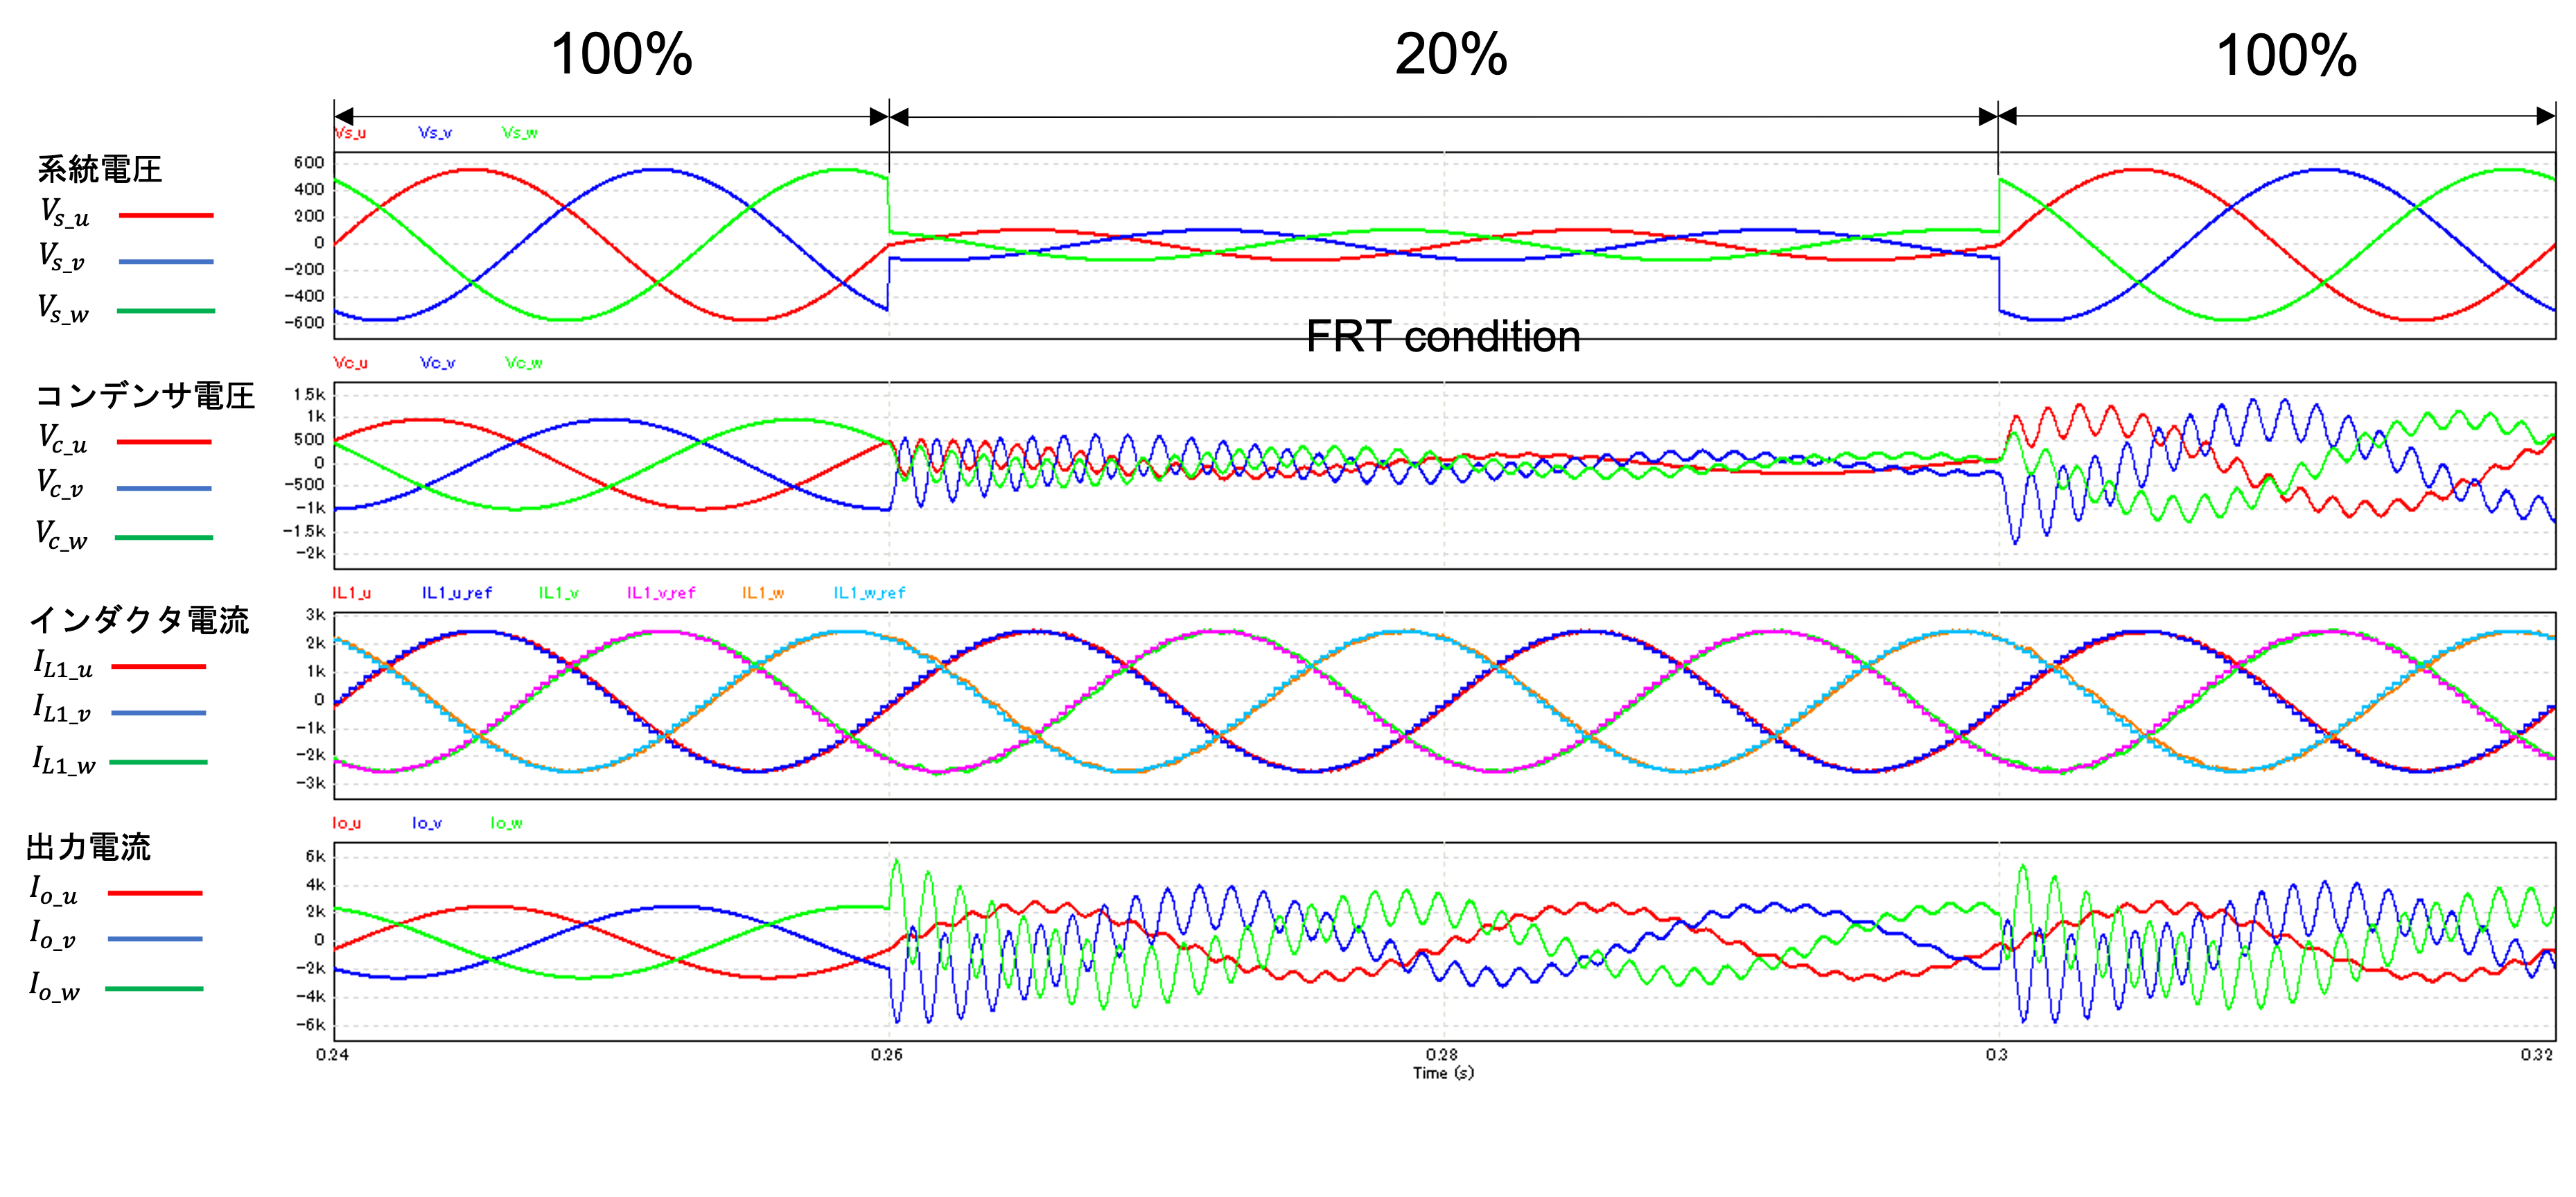
\includegraphics[width=140mm]{image/chapter3/Fig3.2.png}
    \caption{系統擾乱発生時の出力波形}
    \label{Fig3.2}
\end{figure}


表\ref{Tab3.3}にシミュレーション結果を示す．
\begin{table}[htb]
\centering
  \caption{シミュレーション結果}
  \begin{tabular}{c|c|c|c}  \hline\hline 
    \multirow{2}{*}{Condition}& \multicolumn{3}{|c}{THD [\%]} \\  \cline{2-4}
     & U相 & V相  & W相\\  \hline 
    定常時 & 0.88 & 0.90 & 0.93 \\ 
    系統擾乱発生時 & 0.77 & 1.02 & 1.17 \\ \hline
  \end{tabular}
  \label{Tab3.3}
\end{table}

表\ref{Tab3.3}より，定常運転時に対して系統擾乱発生時でTHDがそれぞれ，U相で13\%減少，V相で13\%増加，W相で25\%で増加していることがわかる．\\
外乱補償型マルチサンプリングデッドビート制御の定常運転時と系統擾乱発生時の出力応答を示す．

\begin{figure}[ht]
    \center
    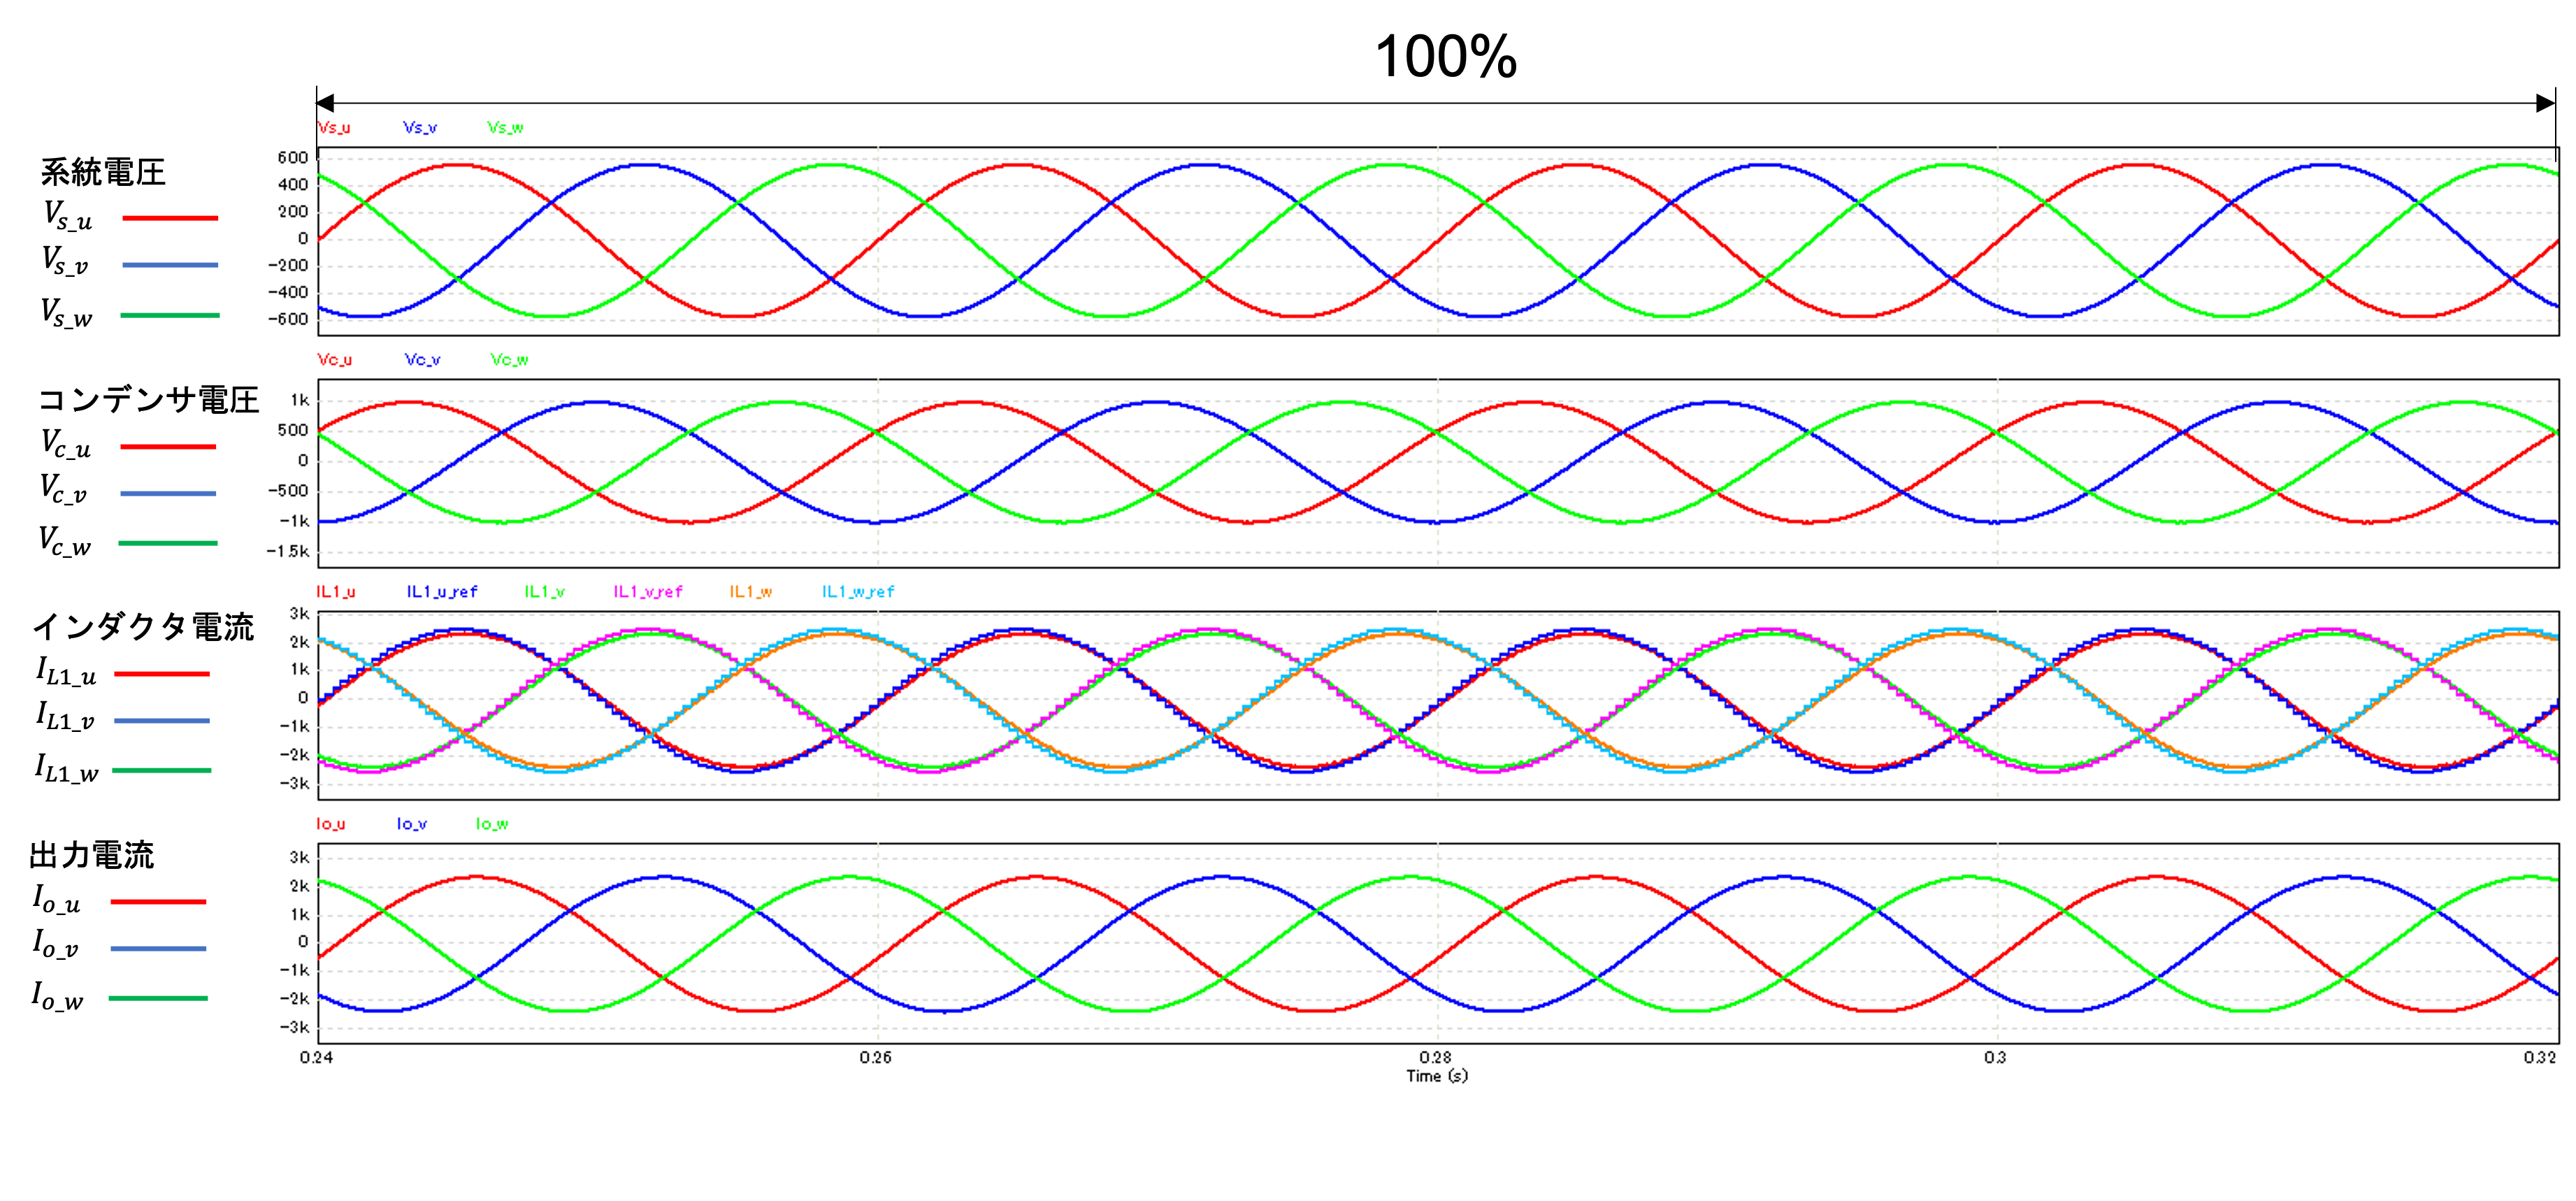
\includegraphics[width=140mm]{image/chapter3/Fig3.3.png}
    \caption{定常運転時の出力波形}
    \label{Fig3.3}
\end{figure}

\begin{figure}[ht]
    \center
    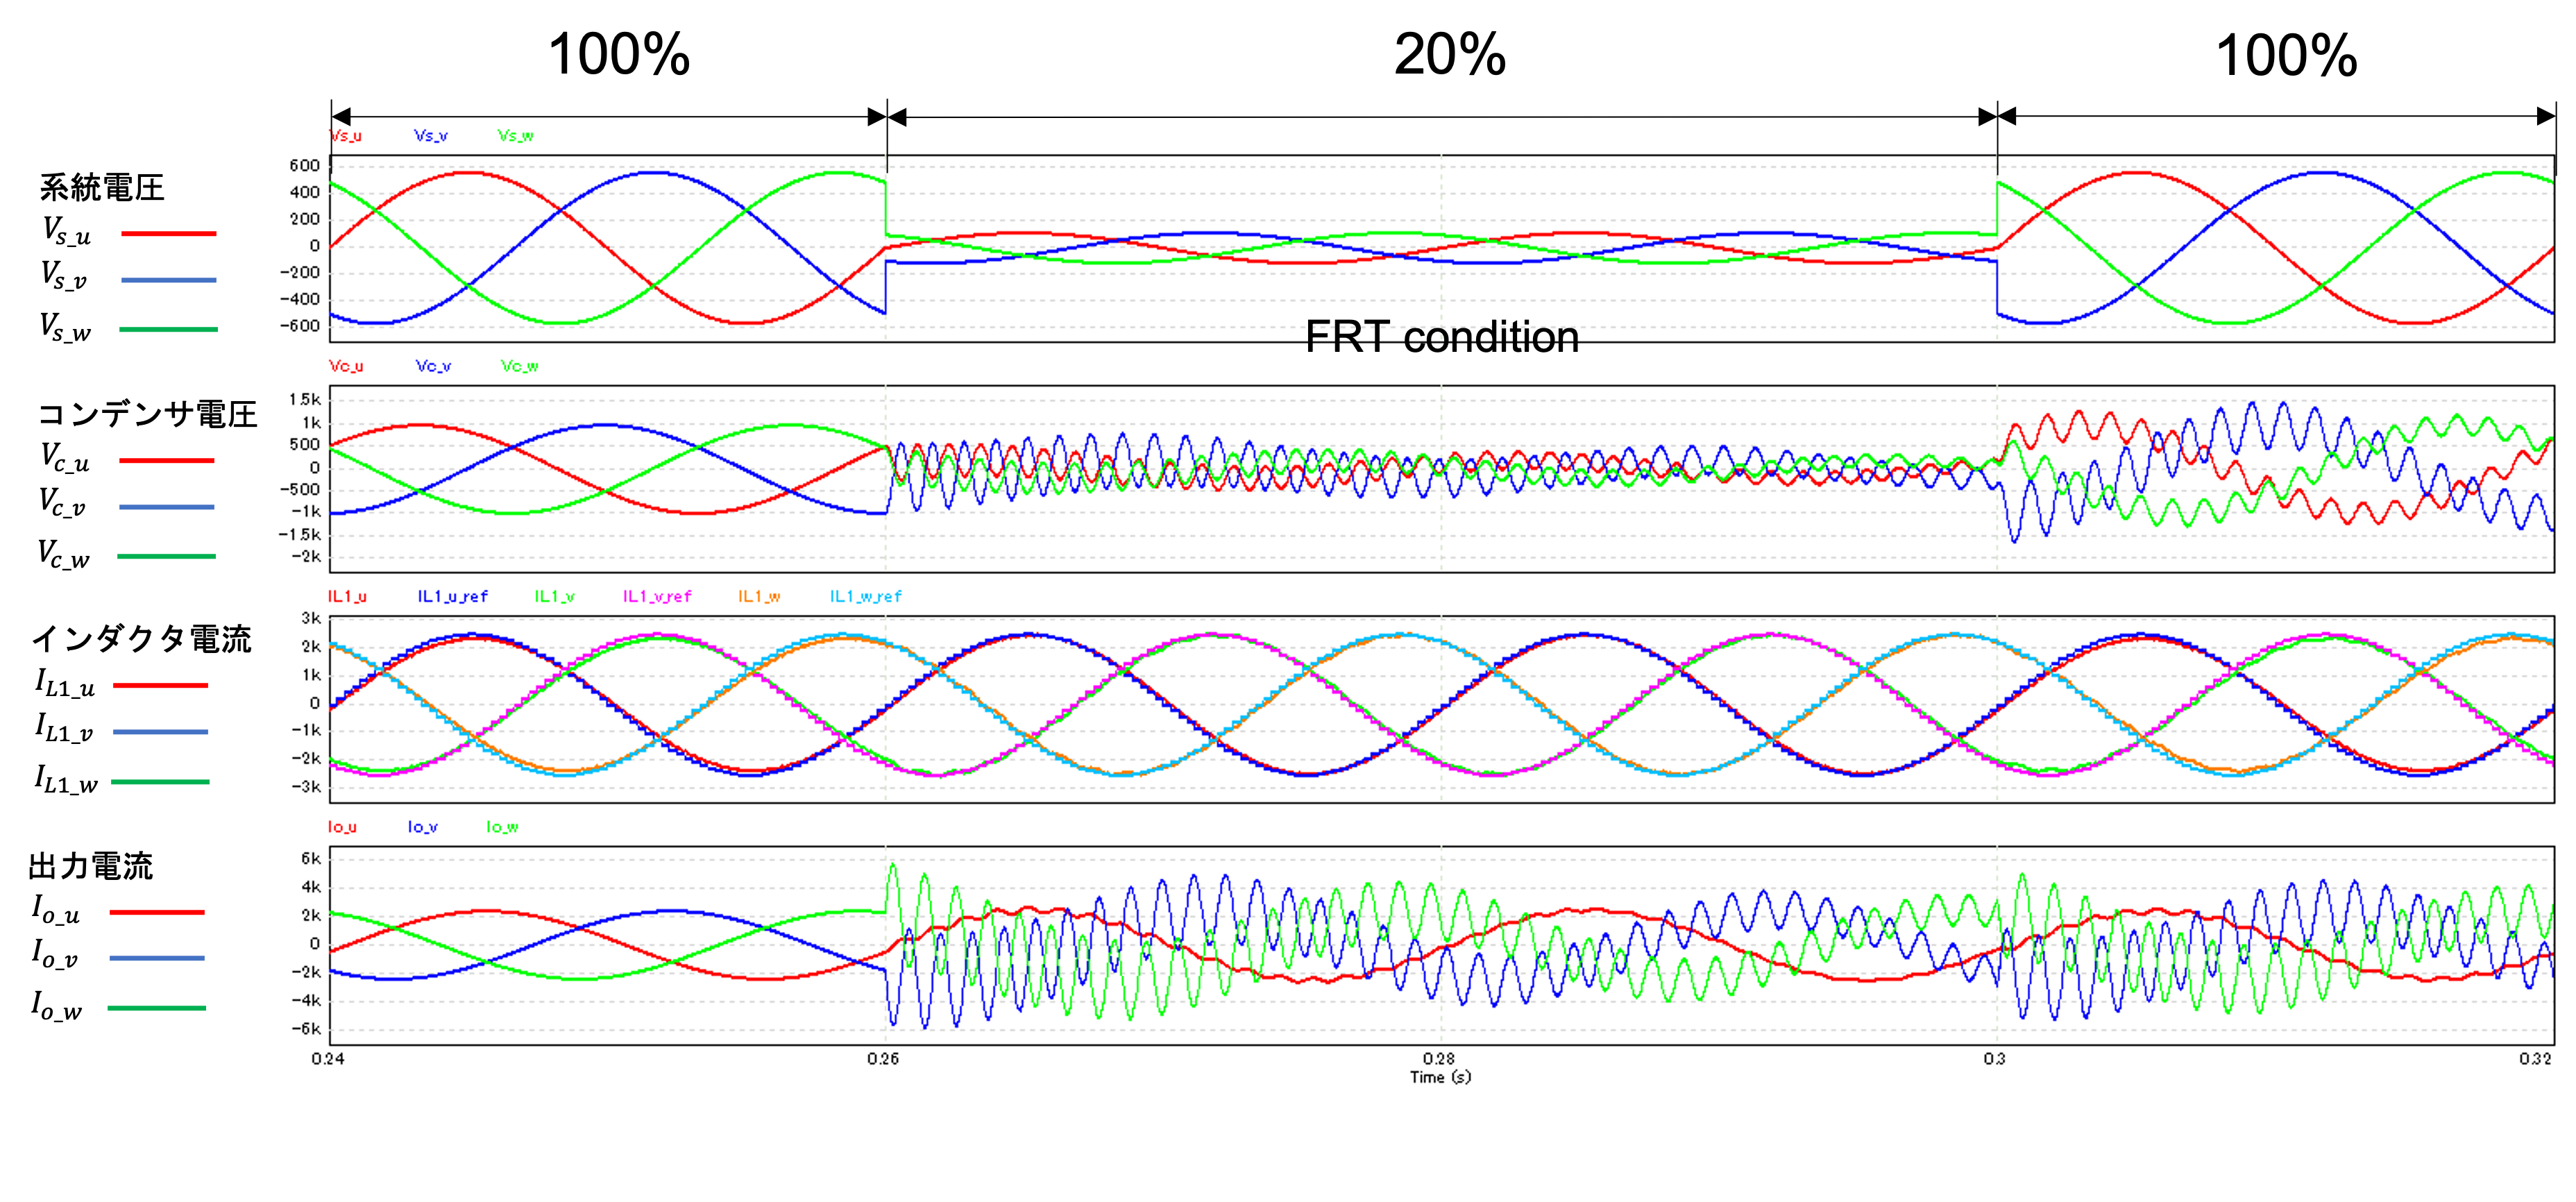
\includegraphics[width=140mm]{image/chapter3/Fig3.4.png}
    \caption{系統擾乱発生時の出力波形}
    \label{Fig3.4}
\end{figure}

\newpage

表\ref{Tab3.4}にシミュレーション結果を示す．
\begin{table}[htb]
\centering
  \caption{シミュレーション結果}
  \begin{tabular}{c|c|c|c}  \hline\hline 
    \multirow{2}{*}{Condition}& \multicolumn{3}{|c}{THD [\%]} \\  \cline{2-4}
     & U相 & V相  & W相\\  \hline 
    定常時 & 0.89 & 0.88 & 0.88 \\ 
    系統擾乱発生時 & 0.75 & 1.46 & 1.46 \\ \hline
  \end{tabular}
  \label{Tab3.4}
\end{table}

表\ref{Tab3.4}より，定常運転時に対して系統擾乱発生時でTHDがそれぞれ，U相で19\%減少，V相で22\%増加，W相で22\%で増加していることがわかる．\\

\subsection{アンノミナル検証}
パターン1のときの外乱補償型シングルレートデッドビート制御の出力応答波形を示す．
\newpage

\begin{figure}[ht]
    \center
    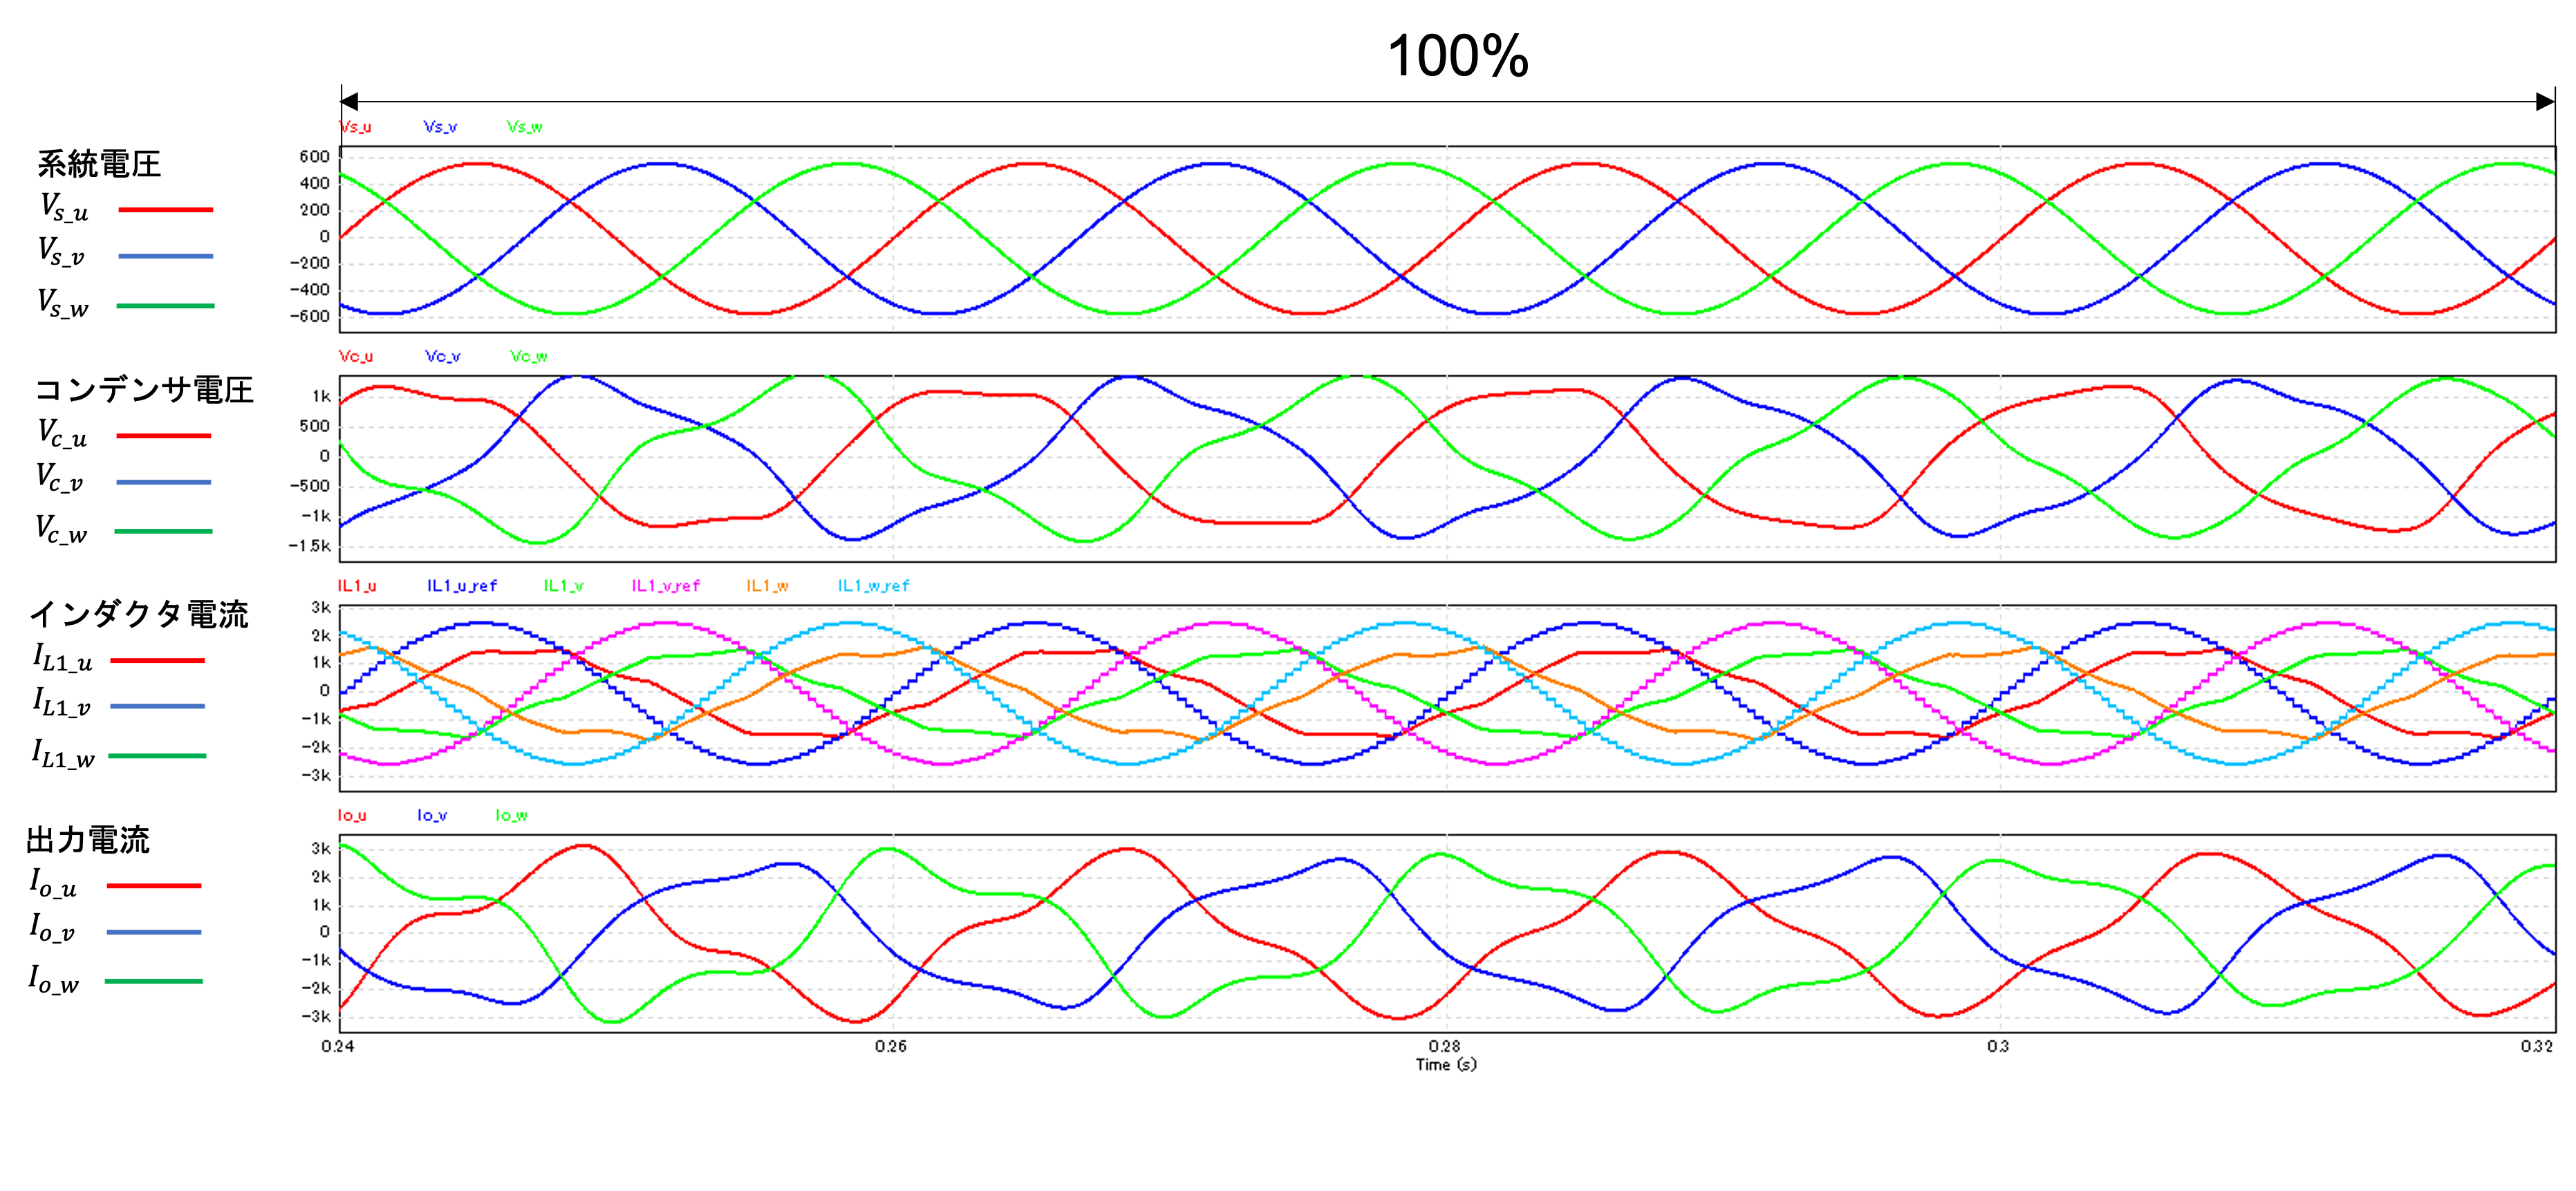
\includegraphics[width=140mm]{image/chapter3/Fig3.5.png}
    \caption{定常運転時(パターン1)}
    \label{Fig3.5}
\end{figure}

\begin{figure}[ht]
    \center
    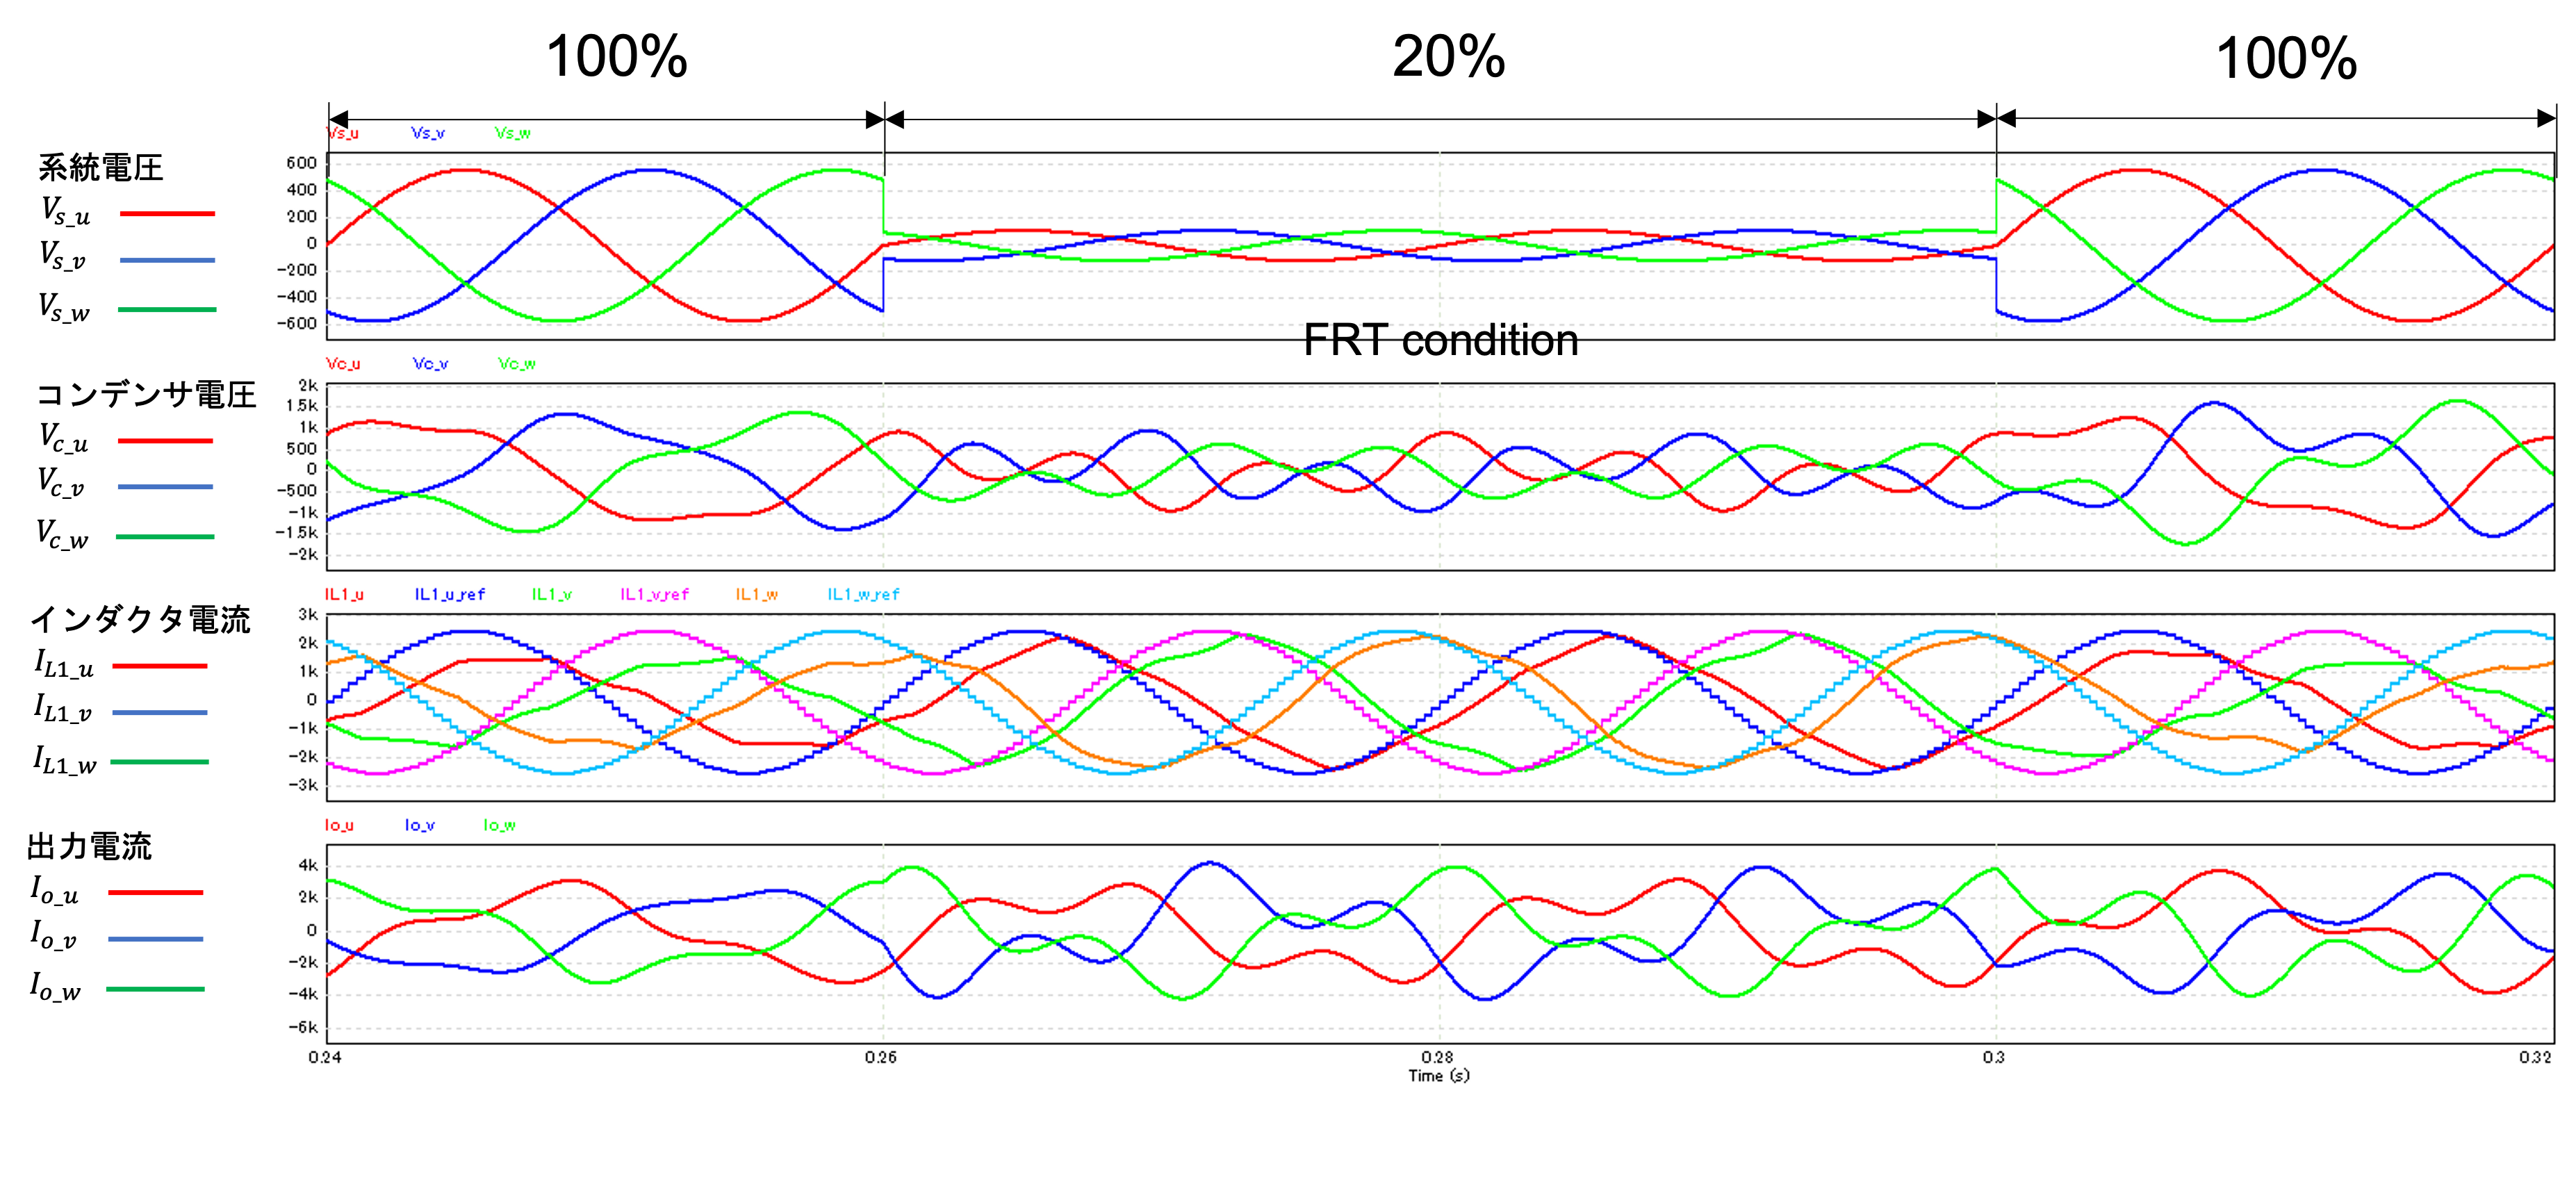
\includegraphics[width=140mm]{image/chapter3/Fig3.6.png}
    \caption{系統擾乱発生時(パターン1)}
    \label{Fig3.6}
\end{figure}

表\ref{Tab3.5}にシミュレーション結果を示す．
\begin{table}[htb]
\centering
  \caption{シミュレーション結果}
  \begin{tabular}{c|c|c|c}  \hline\hline 
    \multirow{2}{*}{Condition}& \multicolumn{3}{|c}{THD [\%]} \\  \cline{2-4}
     & U相 & V相  & W相\\  \hline 
    定常時 & 8.37 & 9.11 & 8.95 \\ 
    系統擾乱発生時 & 7.35 & 8.36 & 7.31 \\ \hline
  \end{tabular}
  \label{Tab3.5}
\end{table}

表\ref{Tab3.5}から，定常運転時と系統擾乱発生時の場合において制御量であるインダクタ電流$I_{L1}$を制御することが出来ていないことがわかる．また，THDはFRT要件で定められている5\%を満たしていないことがわかる．定常運転時に対して系統擾乱発生時でTHDがそれぞれU相で12\%減少，V相で8\%減少，W相で18\%減少していることがわかる．\\
パターン2のときの外乱補償型シングルレートデッドビート制御の出力応答波形を示す．

\begin{figure}[ht]
    \center
    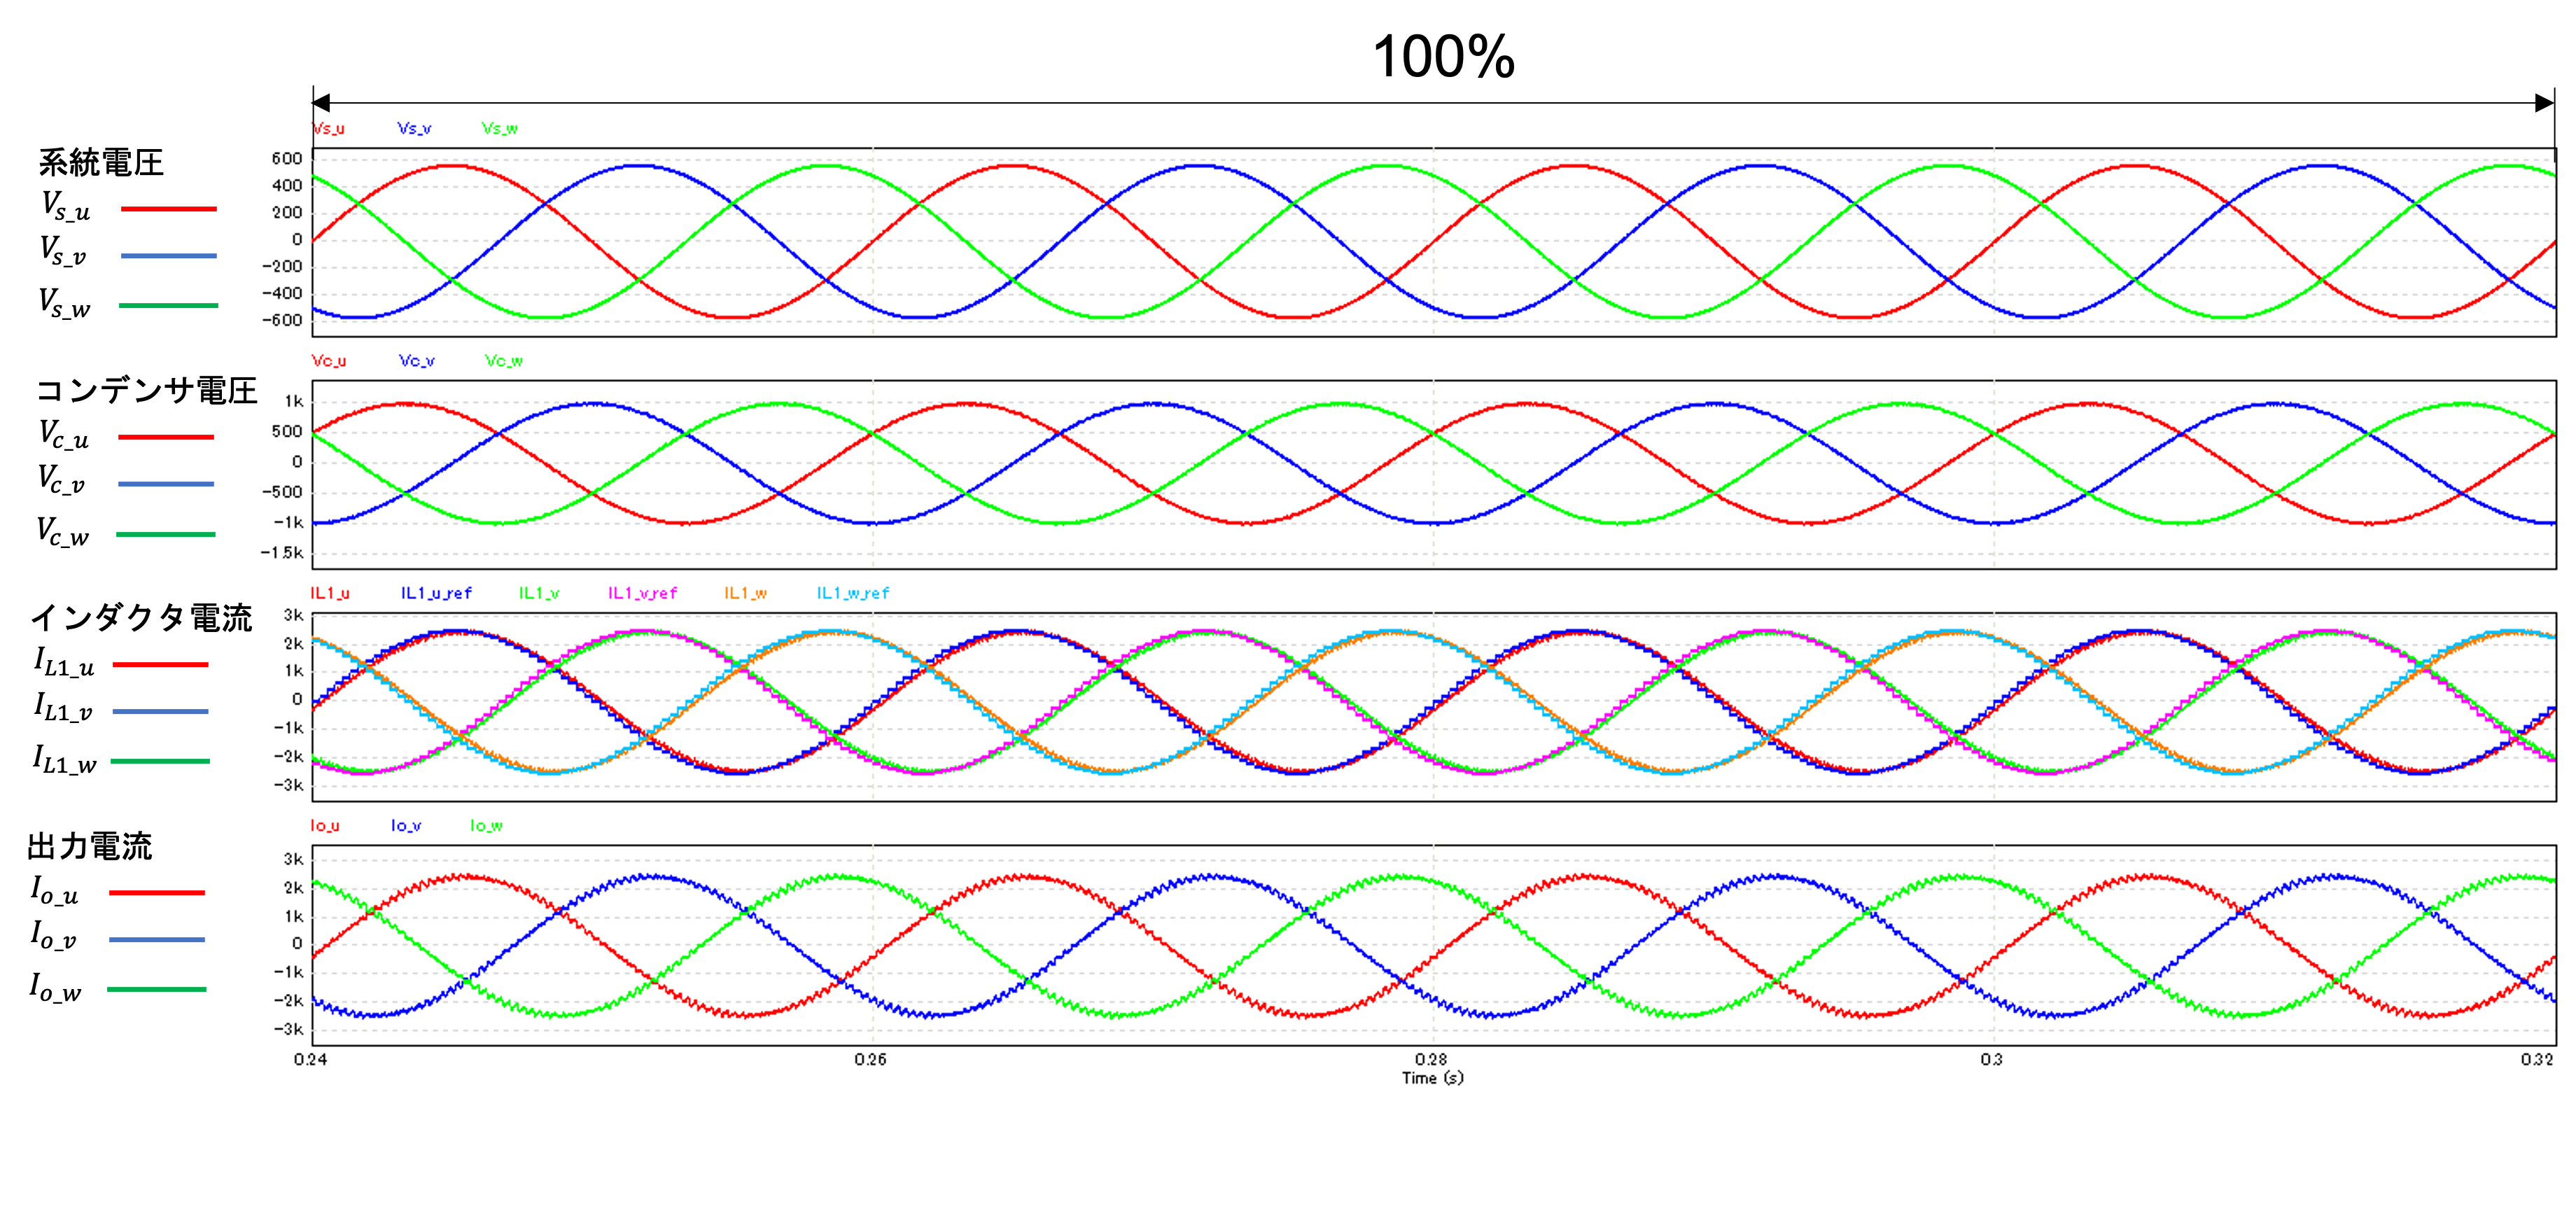
\includegraphics[width=140mm]{image/chapter3/Fig3.7.png}
    \caption{定常運転時(パターン2)}
    \label{Fig3.7}
\end{figure}

\begin{figure}[ht]
    \center
    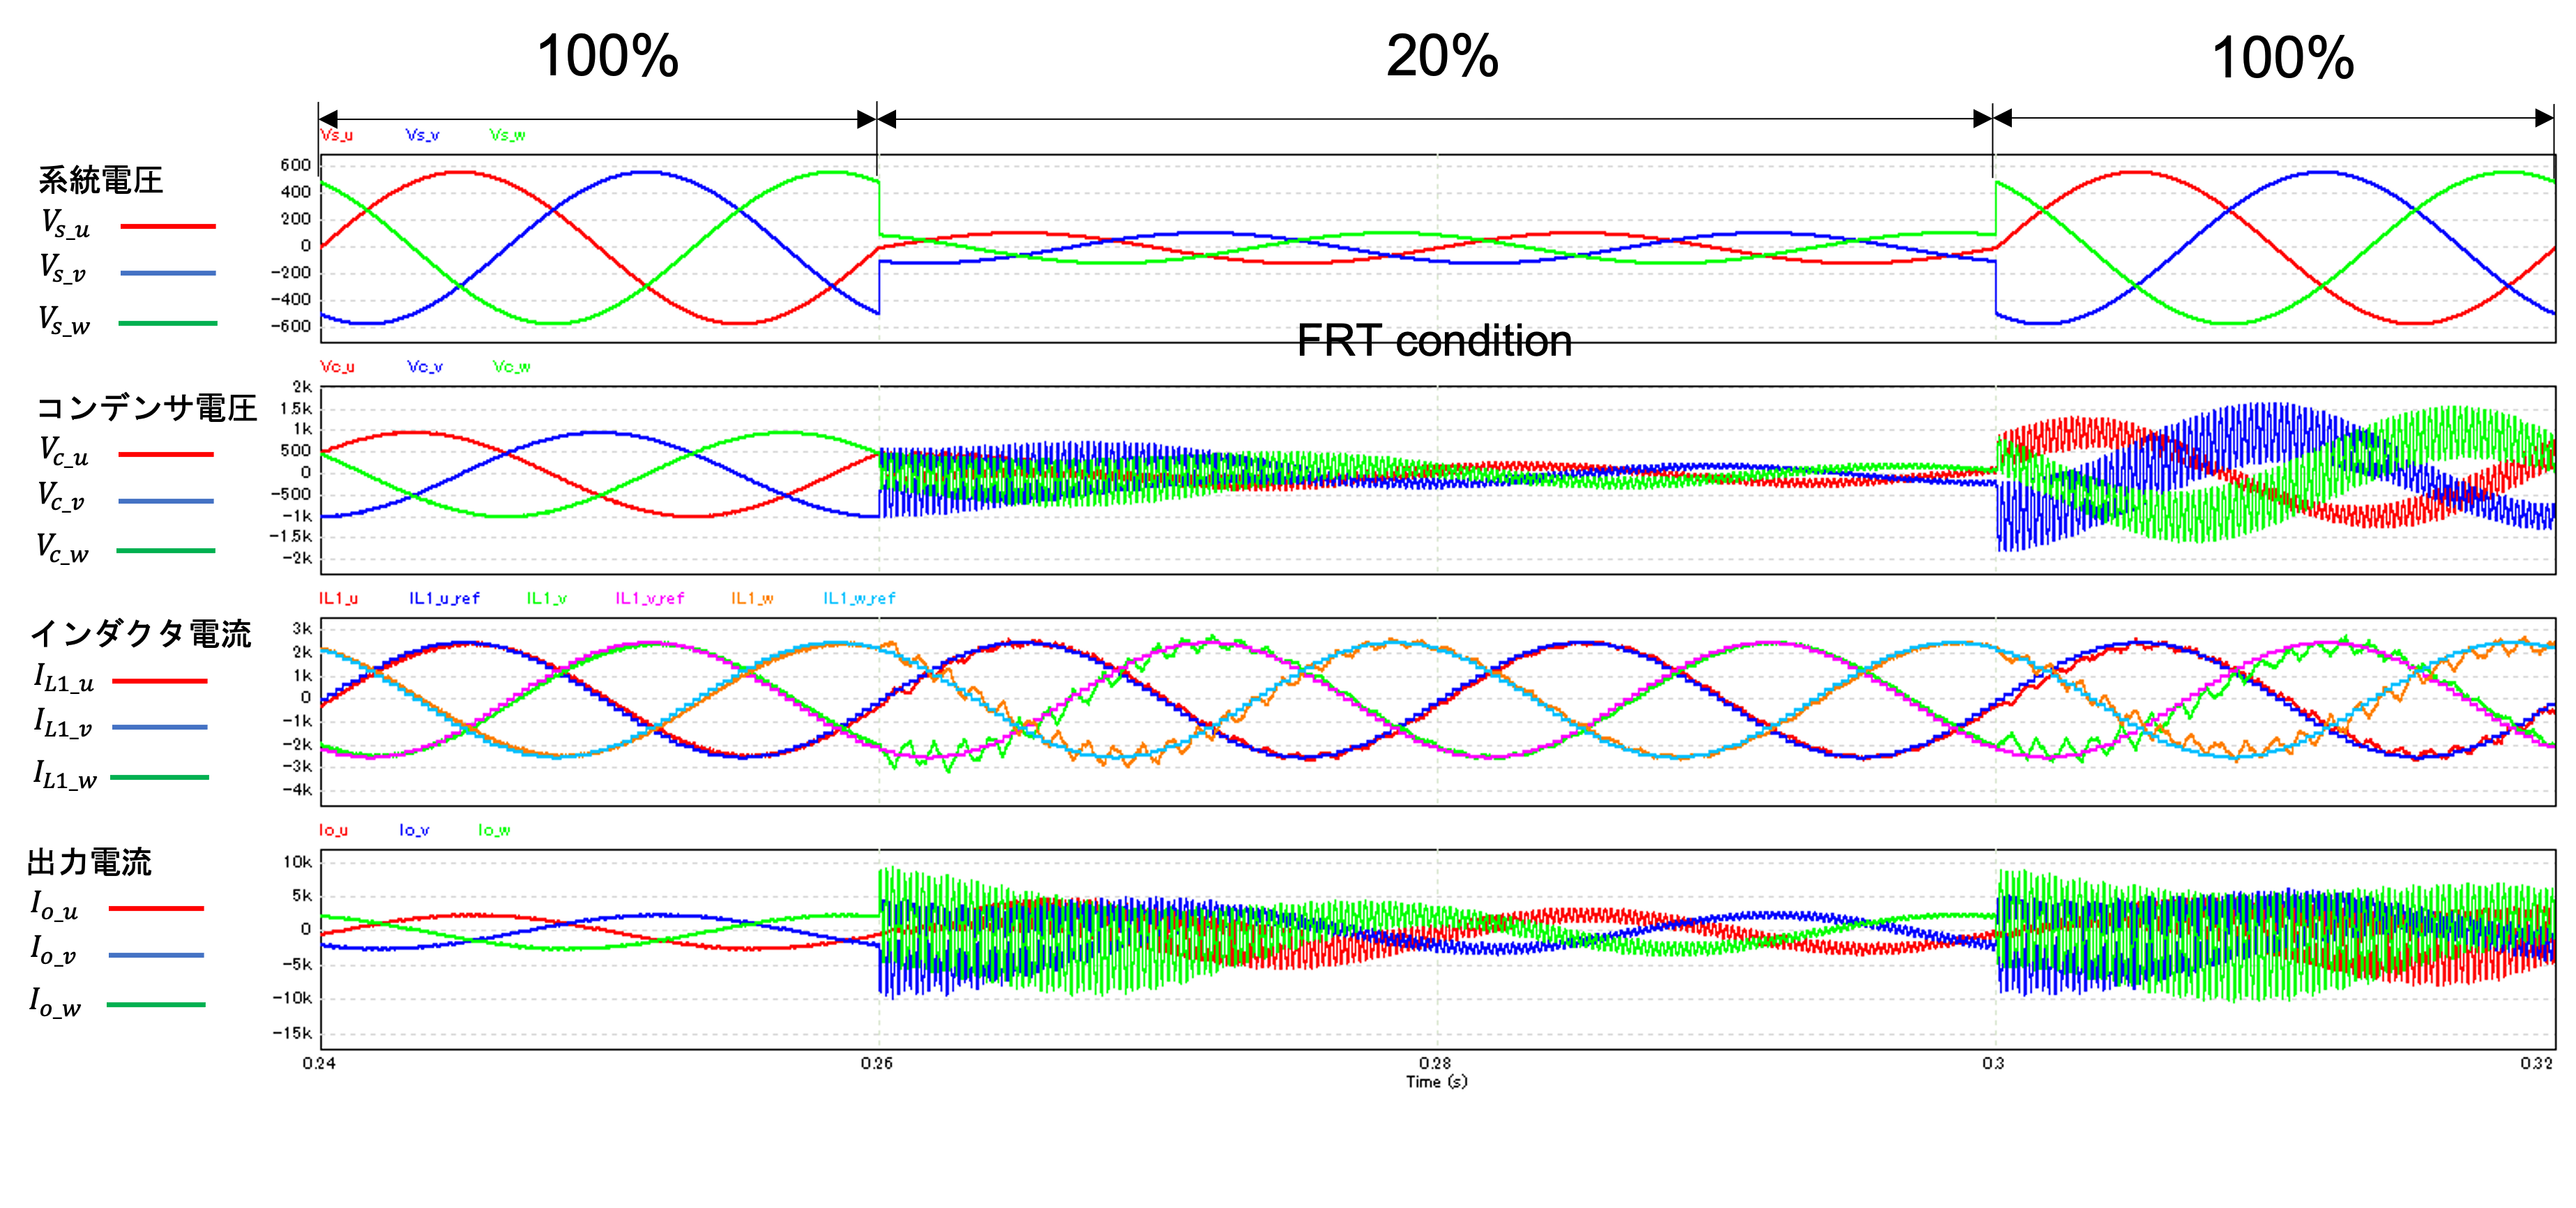
\includegraphics[width=140mm]{image/chapter3/Fig3.8.png}
    \caption{系統擾乱発生時(パターン2)}
    \label{Fig3.8}
\end{figure}

\newpage

表\ref{Tab3.6}にシミュレーション結果を示す．
\begin{table}[htb]
\centering
  \caption{シミュレーション結果}
  \begin{tabular}{c|c|c|c}  \hline\hline 
    \multirow{2}{*}{Condition}& \multicolumn{3}{|c}{THD [\%]} \\  \cline{2-4}
     & U相 & V相  & W相\\  \hline 
    定常時 & 18.4 & 18.5 & 18.6 \\ 
    系統擾乱発生時 & 28.9 & 22.4 & 41.9 \\ \hline
  \end{tabular}
  \label{Tab3.6}
\end{table}

表\ref{Tab3.6}から，定常運転時と系統擾乱発生時の場合において制御量であるインダクタ電流$I_{L1}$を制御することが出来ているわかる．一方で定常運転時，系統擾乱発生時のTHDはFRT要件で定められている5\%を満たしていないことがわかる．常運転時に対して系統擾乱発生時でTHDがそれぞれU相で57\%増加，V相で21\%増加，W相で125\%増加していることがわかる．\\
さらに，コンデンサ電圧$V_{c}$，出力電流$I_{o}$でフィルタ共振を起こしていることが確認できた．

パターン1のときの外乱補償型マルチサンプリングデッドビート制御の出力応答波形を示す．

\begin{figure}[ht]
    \center
    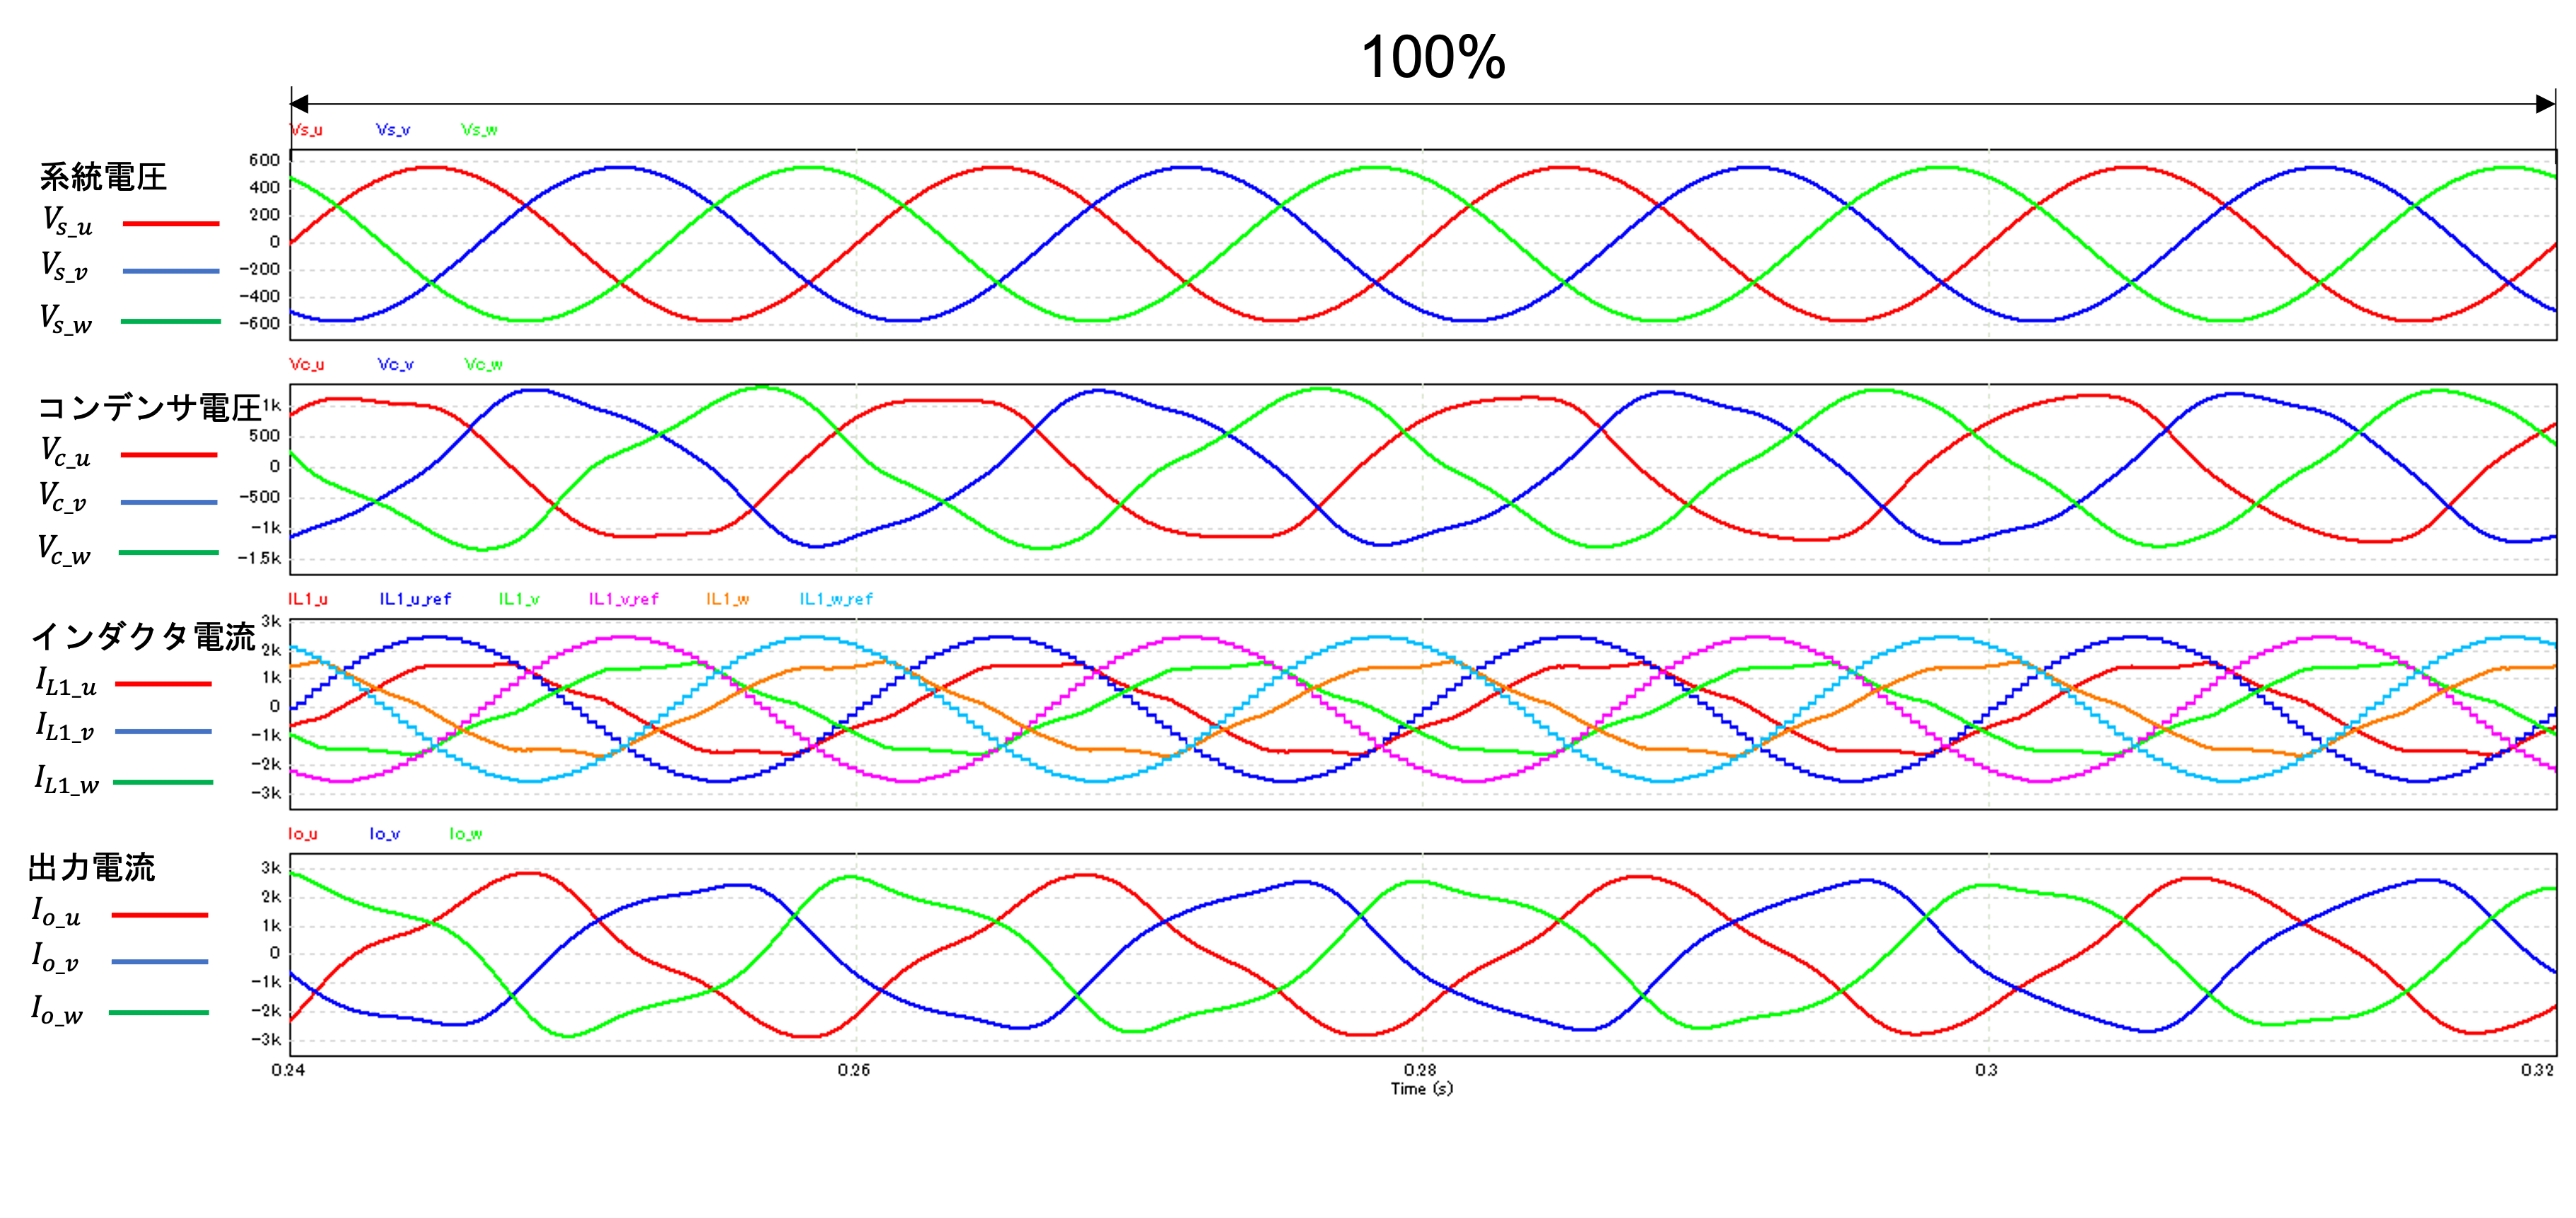
\includegraphics[width=140mm]{image/chapter3/Fig3.9.png}
    \caption{定常運転時(パターン1)}
    \label{Fig3.9}
\end{figure}

\begin{figure}[ht]
    \center
    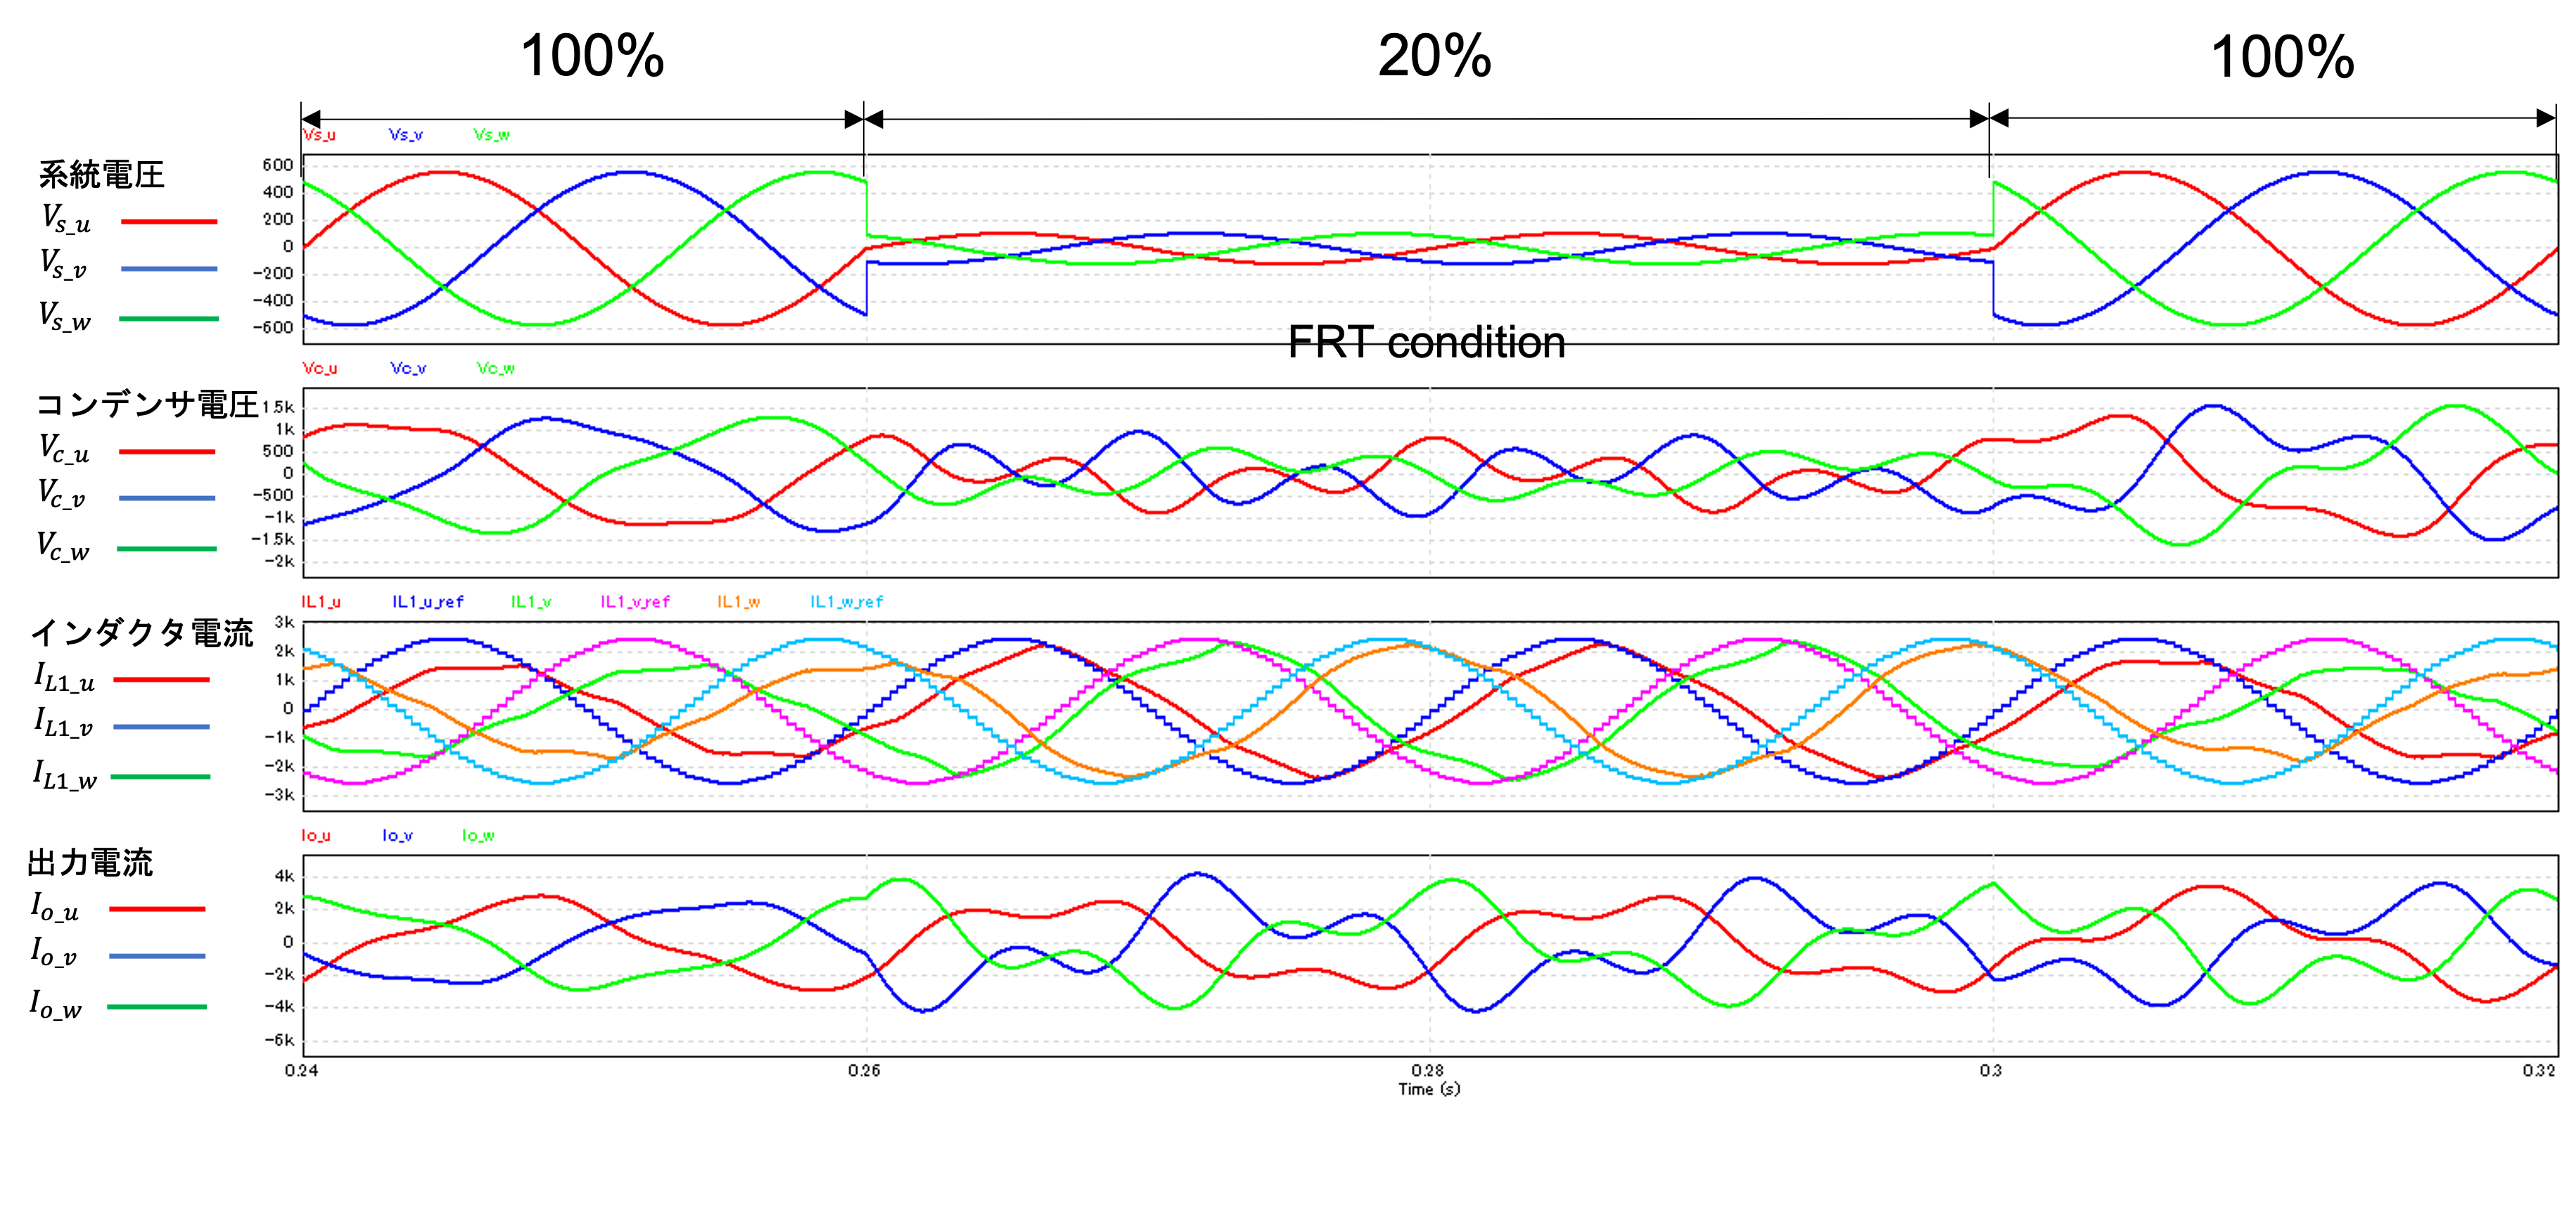
\includegraphics[width=140mm]{image/chapter3/Fig3.10.png}
    \caption{系統擾乱発生時(パターン1)}
    \label{Fig3.10}
\end{figure}

\newpage
表\ref{Tab3.7}にシミュレーション結果を示す．
\begin{table}[htb]
\centering
  \caption{シミュレーション結果}
  \begin{tabular}{c|c|c|c}  \hline\hline 
    \multirow{2}{*}{Condition}& \multicolumn{3}{|c}{THD [\%]} \\  \cline{2-4}
     & U相 & V相  & W相\\  \hline 
    定常時 & 7.40 & 7.76 & 7.75 \\ 
    系統擾乱発生時 & 6.08 & 8.42 & 6.86 \\ \hline
  \end{tabular}
  \label{Tab3.7}
\end{table}

表\ref{Tab3.7}から，定常運転時と系統擾乱発生時の場合において制御量であるインダクタ電流$I_{L1}$を制御することが出来ていないことがわかる．また，THDはFRT要件で定められている5\%を満たしていないことがわかる．定常運転時に対して系統擾乱発生時でTHDがそれぞれU相で18\%減少，V相で9\%増加，W相で11\%減少していることがわかる．\\
パターン2のときの外乱補償型マルチサンプリングデッドビート制御の出力応答波形を示す．

\begin{figure}[ht]
    \center
    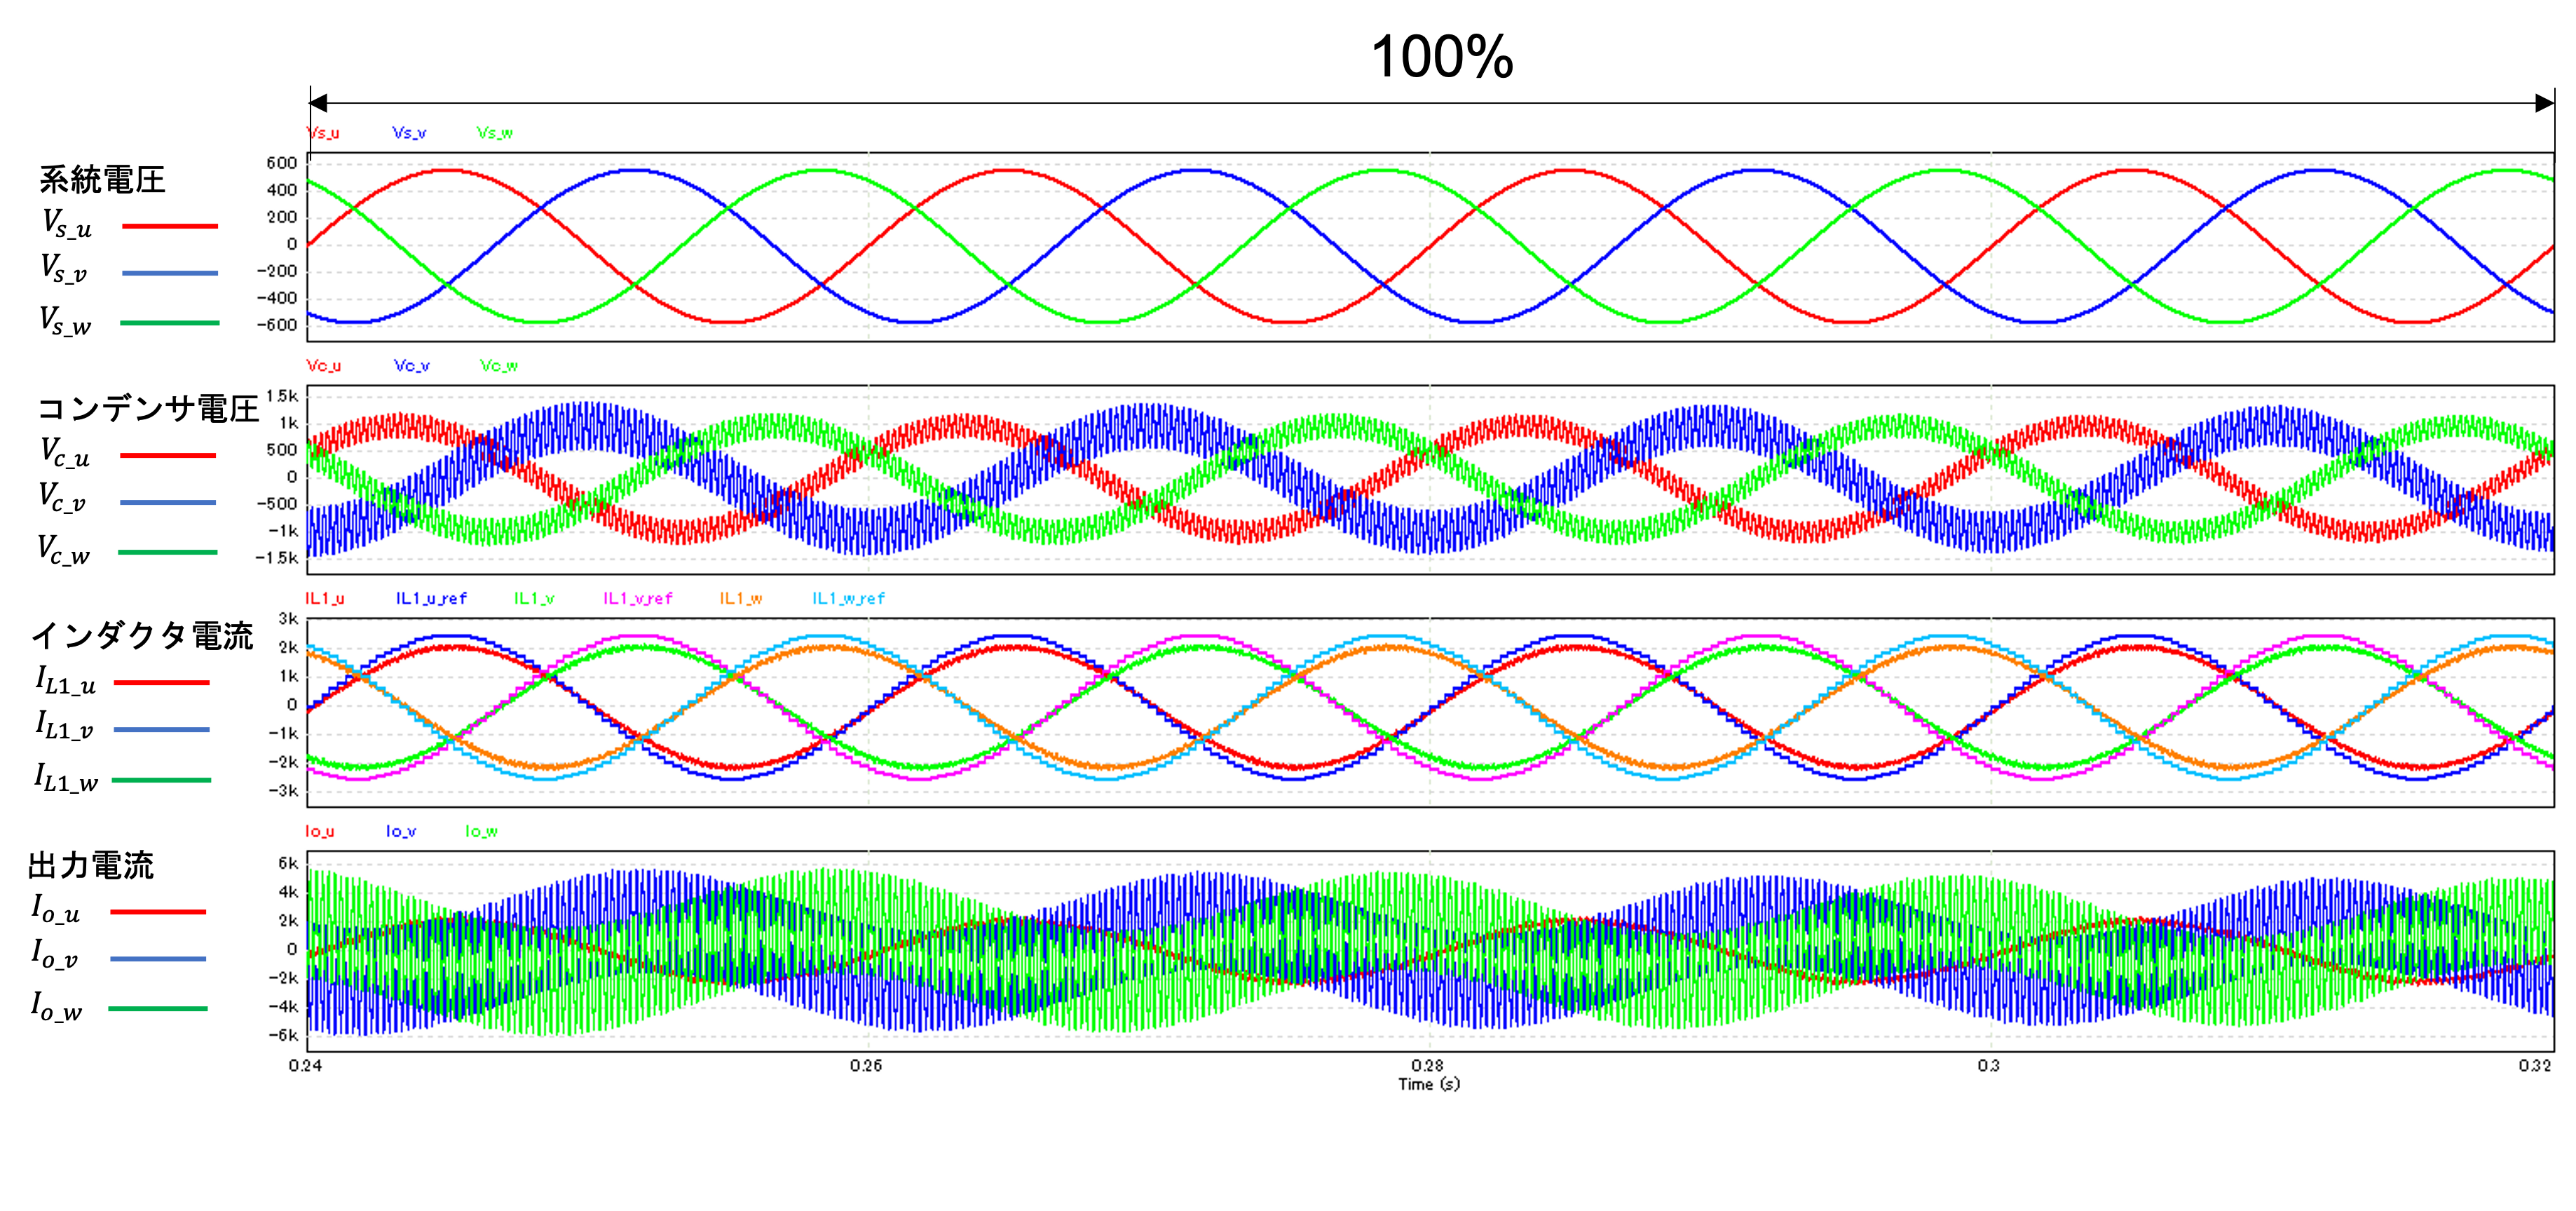
\includegraphics[width=140mm]{image/chapter3/Fig3.11.png}
    \caption{定常運転時(パターン2)}
    \label{Fig3.11}
\end{figure}

\begin{figure}[ht]
    \center
    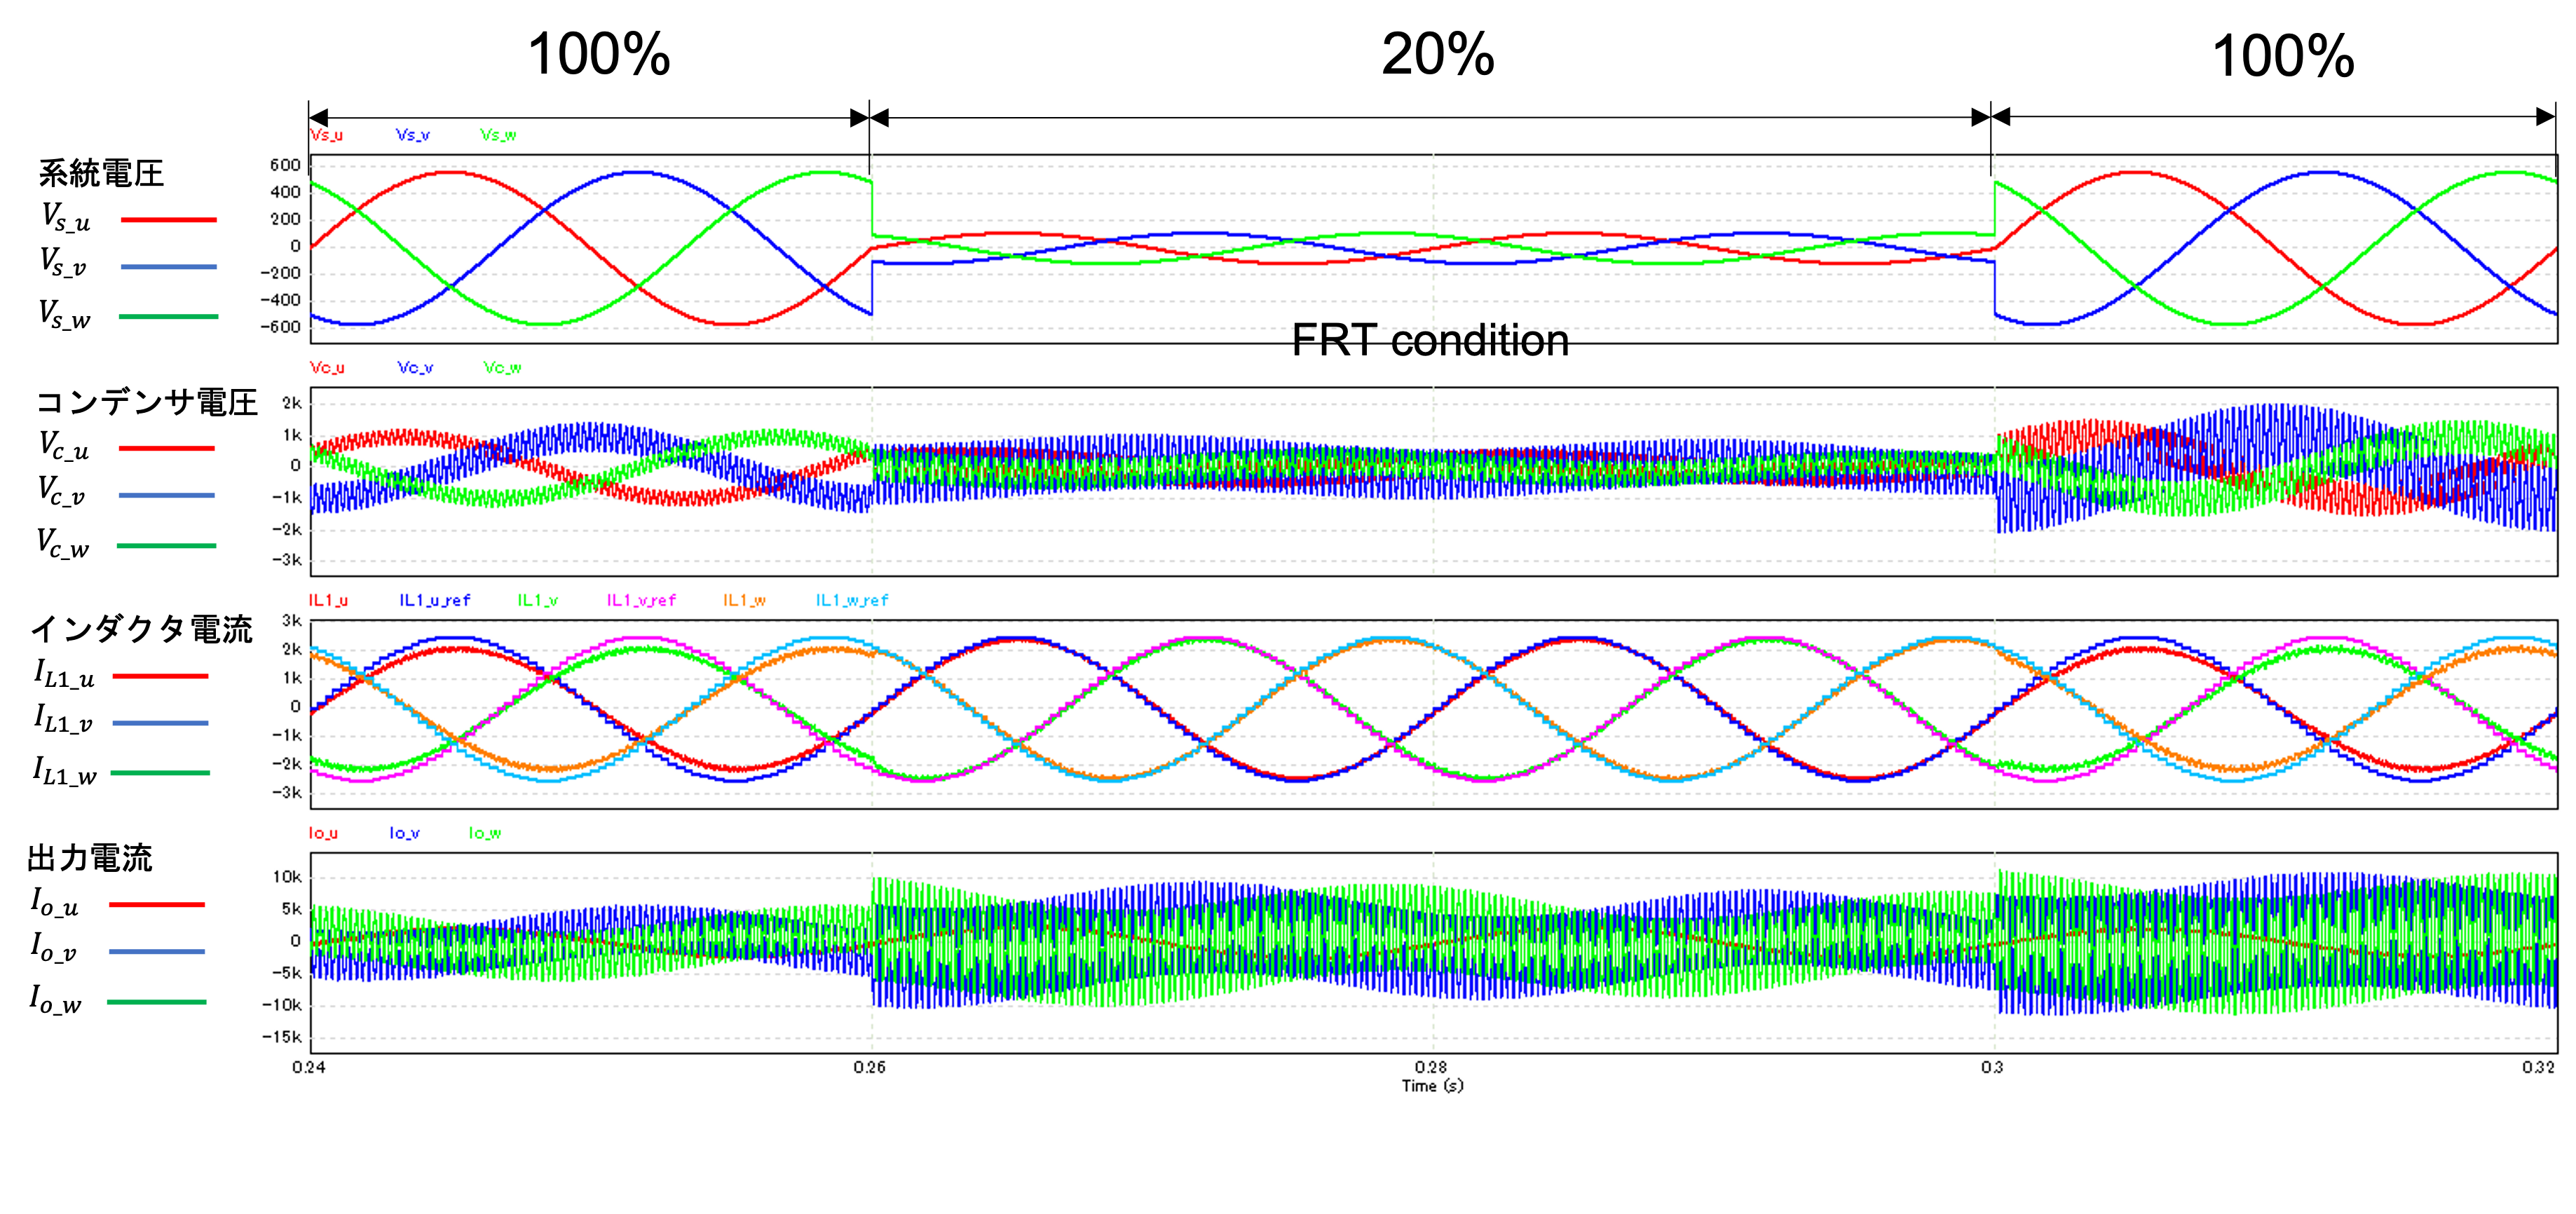
\includegraphics[width=140mm]{image/chapter3/Fig3.12.png}
    \caption{系統擾乱発生時(パターン2)}
    \label{Fig3.12}
\end{figure}

表\ref{Tab3.8}にシミュレーション結果を示す．
\newpage

\begin{table}[htb]
\centering
  \caption{シミュレーション結果}
  \begin{tabular}{c|c|c|c}  \hline\hline 
    \multirow{2}{*}{Condition}& \multicolumn{3}{|c}{THD [\%]} \\  \cline{2-4}
     & U相 & V相  & W相\\  \hline 
    定常時 & 2.09 & 2.29 & 2.31 \\ 
    系統擾乱発生時 & 1.16 & 1.98 & 1.08 \\ \hline
  \end{tabular}
  \label{Tab3.8}
\end{table}

表\ref{Tab3.8}から，定常運転時と系統擾乱発生時の場合において制御量であるインダクタ電流$I_{L1}$を制御することが出来ているわかる．また，定常運転時，系統擾乱発生時のTHDはFRT要件で定められている5\%を満たしていることがわかる．定常運転時に対して系統擾乱発生時でTHDがそれぞれU相で45\%減少，V相で14\%減少，W相で54\%減少していることがわかる．\\
さらに，コンデンサ電圧$V_{c}$，出力電流$I_{o}$でフィルタ共振を起こしていることが確認できた．\par
表\ref{Tab3.9}にシミュレーション結果の一覧を示す．

\begin{table}[htb]
 %\centering
 \footnotesize	
 \small
  \caption{シミュレーション結果の一覧}
  \begin{tabular}{ccc|c|c|c|c}  \hline\hline 
    \multicolumn{2}{c}{\multirow{2}{*}{Condition}}& \multicolumn{3}{|c}{Parameter} & \multicolumn{2}{|c}{THD[\%](U相)}\\ \cline{3-7}
    \multicolumn{2}{c|}{}  &  $L_{1}$ & $C$ & $L2$          & DC-SRDB &DC-MSSRDB \\ \cline{1-7}
    \multirow{2}{*}{ノミナル} &  \multicolumn{1}{|c|}{定常時} & \multirow{2}{*}{$51\mu $H} & \multirow{2}{*}{$995 \mu $F} & \multirow{2}{*}{$51\mu $H}  & 0.88\% & 0.89 \% \\
     & \multicolumn{1}{|c|}{系統擾乱} & & & & 0.77\% & 1.46 \% \\\cline{1-7}
    アンノミナル & \multicolumn{1}{|c|}{-} & - & - & - & - & - \\ 
    \multirow{2}{*}{パターン1} & \multicolumn{1}{|c|}{定常時} &\multirow{2}{*}{1.5 mH}&\multirow{2}{*}{2.0 mF}&\multirow{2}{*}{0.2 mH}&8.37\%&7.40\% \\ 
     &\multicolumn{1}{|c|}{系統擾乱}& & & &7.35\% &6.86\%\\ \cline{1-7}
    \multirow{2}{*}{パターン2} &\multicolumn{1}{|c|}{定常時} &\multirow{2}{*}{0.35 mH}&\multirow{2}{*}{$200 \mu$F}& \multirow{2}{*}{0.02 mH}& 18.4\% &2.09\%\\ 
     &\multicolumn{1}{|c|}{系統擾乱}& & & &28.9\%&1.16\% \\ \hline 
  \label{Tab3.9}
  \end{tabular}
\end{table}


表\ref{Tab3.9}は定常運転時・系統擾乱発生時において，ノミナル，アンノミナル時にDC-SRDB制御，DC-MSSRDB制御を適用した際にTHDがどのように変化するのかを表している．\par
表\ref{Tab3.9}より，ノミナル時は，定常時・系統擾乱発生時のいずれもDC-SRDB制御の方がDC-MSSRDB制御より優れた制御応答を示していることがわかる．一方で，アンノミナル時のパラメータを大きくしたパターン1において定常時，系統擾乱発生時のいずれにおいてもDC-MSSRDB制御の方が優れた制御応答を示していることがわかる．また，パラメータを小さくしたパターン2においても定常時，系統擾乱発生時のいずれの場合でもDC-MSSRDB制御の方が優れた応答性示している．\par
アンノミナル状態のパターン1より，パターン2の方がDC-MSSRDB制御を適用した効果が大きくなっていることがわかる．原因としては，図\ref{Fig3.5}から図\ref{Fig3.12}より，パターン1では，制御対象であるインダクタ電流$I_{L1}$を制御できていないということ，インダクタ，コンデンサのパラメータが制御対象の安定領域から外れたということなどが考えられる．

% 図
% \begin{figure}[htb]
%  \begin{center}
%  \includegraphics[width=50mm]
%  {image/image1}
%  \caption{}
%  \label{fig:}
%  \end{center}
% \end{figure}

% 表
% \begin{table}[htb]
%  \centering
%  \caption{}
%  \label{tab:}
%  \begin{tabular}{c|c}
%   \hline\hline
%   &\\ \hline
%   &\\ \hline
%  \end{tabular}
% \end{table}

% 式
% \begin{eqnarray}
%  a=b \nonumber \\
%  c=d \label{for:}
% \end{eqnarray}

% ソース
% \lstinputlisting[
%   caption=, 
%   label=list:
% ]
% {source/code1}

